\documentclass[oneside]{book}
\tracingstats=1
\usepackage{lal,alltt,array,fancyhdr,geometry,graphicx,color,hyperref,makeidx,wrapfig}
\includeonly{%
  std,%
  support,%
  tools,%
  sample,%
  hello,%
  factories,%
  vectorops,%
  utilities,%
  stats,%
  inject,%
  date,%
  tdfilter,%
  window,%
  fft,%
  clremoval,%
  stochastic,%
  inspiral,%
  noisemodels,%
  bank,%
  ring,
  pulsar,%
  houghpulsar,%
  fct,%
  framedata,%
  comm,%
  findchirp,%
  burstsearch,%
  tfclusters,%
  slopefilters,%
  waveburst,%
  block%
  }


%define page size
%\setlength{\textheight}{9.0in}
%\setlength{\textwidth}{6.0in}
%\setlength{\topmargin}{-0.00in}
%\setlength{\oddsidemargin}{-0.25in}
%\setlength{\evensidemargin}{\oddsidemargin}
\geometry{letterpaper,tmargin=0.5in,headheight=0.2in,headsep=0.3in,hmargin=1in}
\sloppy

\pagestyle{fancy}
\fancyhf{}
\lhead{\bf\nouppercase\rightmark}
\rhead{ \bf Pg \thepage}

\makeindex

\newfont{\lsdfont}{cmbx10 at 72pt}
\def\rcs#1{\def\next##1#1{\mbox{##1}}\next}


\begin{document}

\frontmatter

% \reversemarginpar
% \let\marginpar\mparorig
% \providecommand{\marginpar}[1]{\mbox{}\mparorig{\raggedleft\hspace{0pt}#1}}

% The title page:
\title{
%\vspace*{-1.0in}
\sffamily\bfseries\Huge
\textcolor{red}{\lsdfont L}AL
\raisebox{-2.5ex}{\textcolor{green}{\lsdfont S}\hspace{-0.1em}oftware}
\hspace{-2em}
\raisebox{-0.5ex}{\textcolor{blue}{\lsdfont D}\hspace{-0.2em}ocumentation}\\[\bigskipamount]
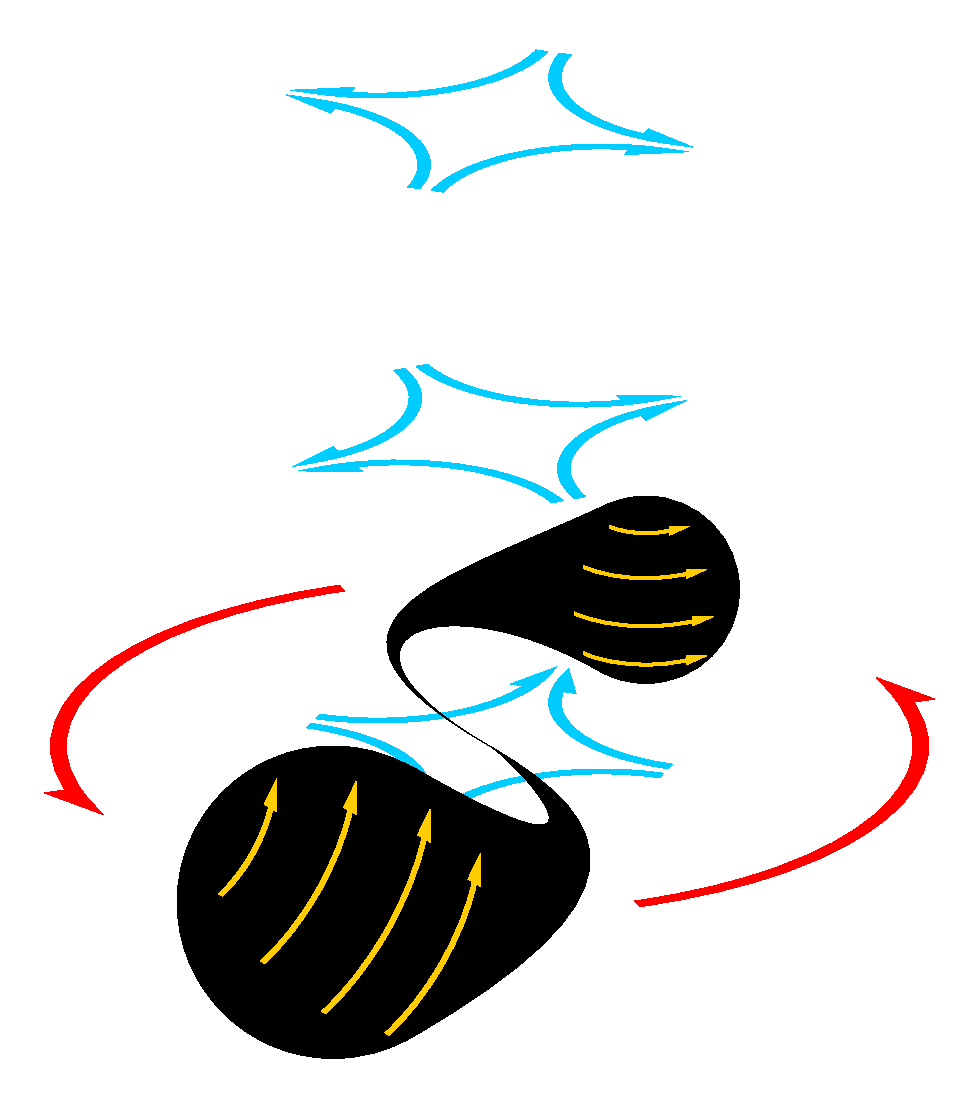
\includegraphics[height=5in]{merger}
}
\author{Contact: Jolien Creighton (Librarian) \texttt{jolien@gravity.phys.uwm.edu}}
\date{RCS \rcs$Revision$\rcs$Date$UTC --- Compiled:
\number\year/\ifnum\month<10 0\fi\number\month/\ifnum\day<10 0\fi\number\day}

\maketitle

\pdfbookmark{Contributors}{aut}
\section*{Contributors}
\begin{verse}
%\input{AUTHORS}
\end{verse}


% The table of contents.
\newpage
\pdfbookmark{Table of Contents}{toc}
\nopagebreak
\tableofcontents


\chapter{Preface}

\bigskip
{\bf {\Huge{Preface to the first edition:}}}

\medskip
\noindent
The formal document governing the LAL-code and documentation is the
{\bf LIGO Data Analysis System Numerical Algorithms Library
Specification and Style Guide}
\verb@http://www.ligo.caltech.edu/docs/T/T990030-07.pdf@ (called the
LAL-Spec through out).  Like a constitution describing a government,
the guidelines given in the LAL-Spec are quite general. What is given
in this document  is a more like the criminal code: the nut-n-bolts
explanation of how to put the LAL-Spec into practice.  Like a
constitution, {\bf if there are any inconsistencies,  the LAL-Spec
takes precedence over any statements in this document.} Also like a
constitution, the LAL-Spec is to be taken very seriously, but it is
not suicide pact: if there are real problems with the Spec, there is a
formal process to change it.

The first part of this document gives a brief introduction to the LAL
and some coding and documentation instructions.  The second part is
the documentation of the LAL code itself.

\bigskip

\bigskip
\noindent
{\bf {\Huge{Preface to the second edition:}}}

\medskip
\noindent
By necessity, the first edition of the
{{\textcolor{red}{\bf L}} {\textcolor{green}{\bf S}} {\textcolor{blue}{\bf D}} }
contained long lists of instructions that specified the layout
of the documentation and code; however many of these rules have
migrated to the LAL-Spec itself, and thus there is less need for
such rules.  Furthermore, now there is a much
larger body of example code  to help guide people in how to
follow the LAL rules.  Therefore Part I of this new edition of
the
{{\textcolor{red}{\bf L}} {\textcolor{green}{\bf S}} {\textcolor{blue}{\bf D}} }
is considerably shorter than its predessor.


\mainmatter

\book{User Guide}
\part{LAL Standard Package}
\chapter{Package \texttt{std}}

This package contains headers providing basic datatypes, constants,
and macros that support the LAL standard.

\newpage\input{LALStdlibH}
\newpage\input{LALRCSIDH}
\newpage\input{LALDatatypesH}
\newpage\input{LALStatusMacrosH}
\newpage\input{LALConstantsH}
\newpage\input{LALStdioH}
\newpage\input{LALVersionH}
\newpage\input{LALMallocH}
\newpage\input{LALErrorH}
\newpage\input{LALGSLH}
\newpage\input{StringInputH}


\newpage\begin{thebibliography}{0}
\bibitem{Barnet:1996}
  Particle Data Group, R.~M. Barnett et al., Phys. Rev. D\textbf{54},
  1 (1996)
\bibitem{Lang:1992}
  K.~R. Lang, \textit{Astrophysical Data: Planets and Stars}.
  Springer-Verlag, New York (1992)
\end{thebibliography}

\chapter{Package \texttt{sample}}

This package contains templates for LAL headers and modules, as well
as a fully-autodocumenting example program based on the primer in the
\verb@std@ package.

\newpage\input{LALSampleH}

\part{General Packages}
%%% Author: David Chin <dwchin@umich.edu> +1-734-730-1274
%%%$Id$

\chapter{Package \texttt{date}}

This package provides routines related to date and time manipulations
(\texttt{Date.h}).  It also provides routines to compute the
difference in time of arrival of a signal at two detector locations,
and also between a detector and the center of the Earth-fixed frame
(\texttt{TimeDelay.h}).

\newpage%%% $Id$

\section{Header \texttt{Date.h}}
\label{sec:dateh:header}
Provides routines for manipulating date and time information.

\subsection{Synopsis}
\label{sec:dateh:synopsis}
\begin{verbatim}
#include "Date.h"
\end{verbatim}

\subsubsection{Datatypes}
\label{sec:dateh:datatypes}
\begin{verbatim}
/* The standard Unix tm structure */
typedef struct
tm
LALUnixDate;

/* This time object is exactly like LIGOTimeGPS, except for the name */
typedef struct
tagLIGOTimeUTC
{
    INT4 utcSeconds;     /* no. of seconds since Unix epoch */
    INT4 utcNanoSeconds; /* residual no. of nanoseconds */
}
LIGOTimeUTC;

/* Encode timezone information */
typedef struct
tagLALTimezone
{
    INT4 secondsWest; /* seconds West of UTC */
    INT4 dst;         /* Daylight Savings Time correction to apply */
}
LALTimezone;    

/* Date and time structure */
typedef struct
tagLALDate
{
    LALUnixDate unixDate;
    INT4        residualNanoSeconds; /* residual nanoseconds */
    LALTimezone timezone;            /* timezone information */
}
LALDate;
\end{verbatim}

\subsubsection{Routine prototypes}
\begin{verbatim}

void JulianDay (Status*, INT4*, const LALDate*);
void ModJulianDay(Status*, REAL8*, const LALDate*);
void JulianDate(Status*, REAL8*, const LALDate*);
void ModJulianDate(Status*, REAL8*, const LALDate*);
void UTCtoGPS(Status*, LIGOTimeGPS*, const LIGOTimeUTC*);
void GPStoUTC(Status*, LIGOTimeUTC*, const LIGOTimeGPS*);
void UTCtime(Status*, LALDate*, const LIGOTimeUTC*);
void DateString(Status*, CHARVector*, const LALDate*);
void GMST1(Status*, REAL8*, const LALDate*, INT4);
void LMST1(Status*, REAL8*, const LALDate*, REAL8, INT4);
void SecsToLALDate(Status*, LALDate*, REAL8);

\end{verbatim}



\subsection{Error conditions}

%%% Local Variables: 
%%% mode: latex
%%% TeX-master: "Date"
%%% End: 


\newpage\input{TimeDelayH}

\newpage\begin{thebibliography}{1}
\expandafter\ifx\csname bibnamefont\endcsname\relax
  \def\bibnamefont#1{#1}\fi
\expandafter\ifx\csname bibfnamefont\endcsname\relax
  \def\bibfnamefont#1{#1}\fi
\expandafter\ifx\csname url\endcsname\relax
  \def\url#1{\texttt{#1}}\fi
\expandafter\ifx\csname urlprefix\endcsname\relax\def\urlprefix{URL }\fi
\providecommand{\bibinfo}[2]{#2}
\providecommand{\eprint}[2][]{\url{#2}}

\bibitem{ptvf:1992}
  W.~H. Press, S.~A. Teukolsky, W.~T. Vetterling, and B.~P. Flannery,
  \textit{Numerical Recipes in C: The Art of Scientific Computing}, 2nd ed.
  (Cambridge University Press, Cambridge, 1992).

\bibitem{fvf:1968}
  Fliegen, and Van~Flandern, \textit{Communications of the ACM}, \textbf{11},
  657, 1968

\bibitem{vfp:1979}
  T.~C. Van Flandern, and K.~F. Pulkkinen,
  \textit{Astrophysical Journal Supplement Series}, \textbf{41},
  391-411, 1979 Nov.

\bibitem{esaa:1992} \textit{Explanatory Supplement to the Astronomical
  Almanac}, P.~K. Seidelmann, \textit{ed.} (University Science Books,
  Mill Valley, 1992)

\bibitem{novas:1999}
  \textit{Naval Observatory Vector Astrometry Subroutines, C Version 2.0.1}
  (U.~S.~Naval Observatory, Astronomical Applications Dept., Dec. 1999)
  \url{http://aa.usno.navy.mil/software/novas/novasUNDERSCOREc/novasc_info.html}

\bibitem{green:1985}
  R.~M. Green, \textit{Spherical Astronomy} (Cambridge University Press,
  Cambridge, 1985)

\bibitem{grasp:194}
  B. Allen, \textit{et al.}, \textit{GRASP: a data analysis package
    for gravitational wave detection} (University of Wisconsin
  - Milwaukee, Milwaukee, 2000)
  \url{http://www.lsc-group.phys.uwm.edu/~ballen/grasp-distribution}

\bibitem{iso8601}
  \textit{International Standard ISO 8601} (International Organization for
  Standardization, Switzerland, 1988, \url{http://www.iso.ch})

\bibitem{ABCF:2000} W.~G. Anderson, P.~R Brady, J.~D.~E. Creighton,
  and \'E.~\'E. Flanagan, \emph{Beam Pattern Response Functions and
  Times of Arrival for Earthbound Interferometers} (2000), unpublished
  Maple worksheet,
  \url{http://dirac.utb.edu/~warren/unprot/beamUNDERSCOREpatternsUNDERSCORE260401.tar.gz}.

\end{thebibliography}

%%% Local Variables:
%%% mode: latex
%%% TeX-master: "main"
%%% End:

%\section{Program \texttt{lalapps\_hello}}
\label{program:lalapps-hello}
\idx[Program]{lalapps\_hello}

\begin{entry}

\item[Name]
\verb$lal_hello$ --- prints ``hello LSC!''

\item[Synopsis]
\verb$lal_hello$ [\verb$-h$] [\verb$-V$] [\verb$-v$]
[\verb$-d$ \textit{dbglvl}] [\verb$-o$ \textit{outfile}]

\item[Description]
\verb$lal_hello$ prints ``hello LSC!'' to the screen or to an output file.

\item[Options]\leavevmode
\begin{entry}
\item[\texttt{-h}]
Print a help message.
\item[\texttt{-V}]
Print the version information.
\item[\texttt{-v}]
Verbose output.
\item[\texttt{-d} \textit{dbglvl}]
Set LAL debug level to \textit{dbglvl}.
\item[\texttt{-o} \textit{outfile}]
Write the output to file \textit{outfile}.
\end{entry}

\item[Debug levels]
The LAL debug level can be specified as an integer or as a string of flags:
\begin{entry}
\item[\texttt{NDEBUG}]
No debugging information is printed and memory debugging code is disabled.
\item[\texttt{ERROR}]
Error messages are printed.
\item[\texttt{WARNING}]
Warning messages are printed.
\item[\texttt{INFO}]
Information messages are printed.
\item[\texttt{TRACE}]
Function call tracing messages are printed.
\item[\texttt{MEMINFO}]
Memory  allocation  information messages are printed.
\item[\texttt{MEMDBG}]
Debugging of memory allocation routines is enabled but no messages are printed.
\end{entry}
The following composite levels are available:
\begin{entry}
\item[\texttt{MSGLVL1}]
Equivalent to \verb$ERROR$
\item[\texttt{MSGLVL2}]
Equivalent to \verb$ERROR | WARNING$
\item[\texttt{MSGLVL3}]
Equivalent to \verb$ERROR | WARNING | INFO$
\item[\texttt{ALLDBG}]
All debugging messages are printed.
\end{entry}

For example, the command
\begin{indented}
\verb$lal_hello -d "ERROR | INFO"$
\end{indented}
will set the debug level so that error and information messages are printed.

\item[Environment]\leavevmode

\begin{entry}
\item[\texttt{LAL\_DEBUG\_LEVEL}]
Default LAL debug level to use.
\end{entry}

\item[Author]
Jolien Creighton

\end{entry}

\chapter{Package \texttt{factories}}

This package provides routines for creating and destroying the LAL aggregate
datatypes.

\newpage\input{AVFactoriesH}
\newpage\input{SeqFactoriesH}

\chapter{Package \texttt{tools}}

This package contains the general purpose LAL tools.

\newpage\input{UnitsH}
\newpage\input{DetectorSiteH}
\newpage\input{DetResponseH}
\newpage\input{CalibrationH}
\newpage\input{ResampleTimeSeriesH}
\newpage\input{LIGOMetadataTablesH}
\newpage\input{LIGOMetadataUtilsH}
\newpage\input{TemplateBankGenerationH}
\newpage\clearpage
\section{Sequence Manipulation}
\label{s:SequenceManipulation}

This is a suite of functions for creating, destroying, and manipulating LAL
sequences.  One pair of functions (the XLAL version and its LAL
counterpart) is available for each method and sequence type.  For example
\texttt{XLALCreateREAL4Sequence()} is available for creating sequences of
\texttt{REAL4} data, and the LAL-stype wrapper
\texttt{LALCreateREAL4Sequence()} is provided which is equivalent to the
XLAL version in all respects except that it adheres to the LAL calling
conventions (eg.\ it takes a \texttt{LALStatus} pointer as its first
argument, its return type is \texttt{void}, etc.).

\subsection{Creation Functions}

\subsubsection{Name}

\texttt{XLALCreate}\textit{sequencetype}\texttt{()},
\texttt{LALCreate}\textit{sequencetype}\texttt{()}

\subsubsection{Synopsis}

\begin{verbatim}
#include <lal/Sequence.h>
\end{verbatim}
\input{SequenceCreateP}

\subsubsection{Description}

These functions create LAL sequences.  The parameter \texttt{length}
specifies the length of the desired sequence.  An XLAL function returns a
pointer to the newly created sequence or \texttt{NULL} on failure.  The LAL
counterpart accepts the address of a pointer which it fills with the
address of the newly created sequence or \texttt{NULL} on failure.
Additionally, the LAL wrapper provides standard LAL-style error checking
via a \texttt{LALStatus} pointer.

\subsubsection{Author}

\verb|Kipp Cannon <kipp@gravity.phys.uwm.edu>|


\subsection{Destruction Functions}

\subsubsection{Name}

\texttt{XLALDestroy}\textit{sequencetype}\texttt{()},
\texttt{LALDestroy}\textit{sequencetype}\texttt{()}

\subsubsection{Synopsis}

\begin{verbatim}
#include <lal/Sequence.h>
\end{verbatim}
\input{SequenceDestroyP}

\subsubsection{Description}

These functions free all memory associated with a LAL sequence.  It is safe
to pass \texttt{NULL} to these functions.

\subsubsection{Author}

\verb|Kipp Cannon <kipp@gravity.phys.uwm.edu>|


\subsection{Cutting Functions}

\subsubsection{Name}

\texttt{XLALCut}\textit{sequencetype}\texttt{()},
\texttt{LALCut}\textit{sequencetype}\texttt{()}

\subsubsection{Synopsis}

\begin{verbatim}
#include <lal/Sequence.h>
\end{verbatim}
\input{SequenceCutP}

\subsubsection{Description}

These functions create a new sequence by extracting a section of an
existing sequence.

\subsubsection{Author}

\verb|Kipp Cannon <kipp@gravity.phys.uwm.edu>|


\subsection{Shrinking Functions}

\subsubsection{Name}

\texttt{XLALShrink}\textit{sequencetype}\texttt{()},
\texttt{LALShrink}\textit{sequencetype}\texttt{()}

\subsubsection{Synopsis}

\begin{verbatim}
#include <lal/Sequence.h>
\end{verbatim}
\input{SequenceShrinkP}

\subsubsection{Description}

These functions reduce the size of an existing sequence.

\subsubsection{Author}

\verb|Kipp Cannon <kipp@gravity.phys.uwm.edu>|

\newpage\clearpage
\section{Frequency Series Manipulation}
\label{s:FrequencySeriesManipulation}

This is a suite of functions for creating, destroying, and manipulating LAL
frequency series.  One pair of functions (the XLAL version and its LAL
counterpart) is available for each method and frequency series type.  For
example \texttt{XLALCreateREAL4FrequencySeries()} is available for creating
frequency series of \texttt{REAL4} data, and the LAL-stype wrapper
\texttt{LALCreateREAL4FrequencySeries()} is provided which is equivalent to
the XLAL version in all respects except that it adheres to the LAL calling
conventions (eg.\ it takes a \texttt{LALStatus} pointer as its first
argument, its return type is \texttt{void}, etc.).

\subsection{Creation Functions}

\subsubsection{Name}

\texttt{XLALCreate}\textit{frequencyseriestype}\texttt{()},
\texttt{LALCreate}\textit{frequencyseriestype}\texttt{()}

\subsubsection{Synopsis}

\begin{verbatim}
#include <lal/FrequencySeries.h>
\end{verbatim}
\input{FrequencySeriesCreateP}

\subsubsection{Description}

These functions create LAL frequency series.  An XLAL function returns a
pointer to the newly created series or \texttt{NULL} on failure.  The LAL
counterpart accepts the address of a pointer which it fills with the
address of the newly created series or \texttt{NULL} on failure.
Additionally, the LAL wrapper provides standard LAL-style error checking
via a \texttt{LALStatus} pointer.

\subsubsection{Author}

\verb|Kipp Cannon <kipp@gravity.phys.uwm.edu>|


\subsection{Destruction Functions}

\subsubsection{Name}

\texttt{XLALDestroy}\textit{frequencyseriestype}\texttt{()},
\texttt{LALDestroy}\textit{frequencyseriestype}\texttt{()}

\subsubsection{Synopsis}

\begin{verbatim}
#include <lal/FrequencySeries.h>
\end{verbatim}
\input{FrequencySeriesDestroyP}

\subsubsection{Description}

These functions free all memory associated with a LAL frequency series.  It
is safe to pass \texttt{NULL} to these functions.

\subsubsection{Author}

\verb|Kipp Cannon <kipp@gravity.phys.uwm.edu>|


\subsection{Cutting Functions}

\subsubsection{Name}

\texttt{XLALCut}\textit{frequencyseriestype}\texttt{()},

\subsubsection{Synopsis}

\begin{verbatim}
#include <lal/FrequencySeries.h>
\end{verbatim}
\input{FrequencySeriesCutP}

\subsubsection{Description}

These functions create a new frequency series by extracting a section of an
existing frequency series.

\subsubsection{Author}

\verb|Kipp Cannon <kipp@gravity.phys.uwm.edu>|


\subsection{Resizing Functions}

\subsubsection{Name}

\texttt{XLALResize}\textit{frequencyseriestype}\texttt{()},
\texttt{XLALShrink}\textit{frequencyseriestype}\texttt{()},
\texttt{LALShrink}\textit{frequencyseriestype}\texttt{()}

\subsubsection{Synopsis}

\begin{verbatim}
#include <lal/FrequencySeries.h>
\end{verbatim}
\input{FrequencySeriesShrinkP}

\subsubsection{Description}

These functions resize an existing frequency series.  The new frequency
series will have the given length, and its contents will consist of that
part of the original time series that started at sample \texttt{first}.  If
\texttt{first} is negative, then the new time series is padded at the start
by that many samples.  The frequency series' heterodyne frequency,
\(f_{0}\), is adjusted appropriately.

The ``Shrink'' functions accept non-negative values for the parameter
\texttt{first}, and are retained only for historical purposes.  New code
should use the ``Resize'' variants.

\subsubsection{Author}

\verb|Kipp Cannon <kipp@gravity.phys.uwm.edu>|


\subsection{Addition Functions}

\subsubsection{Name}

\texttt{XLALAdd}\textit{frequencyseriestype}\texttt{()}

\subsubsection{Synopsis}

\begin{verbatim}
#include <lal/FrequencySeries.h>
\end{verbatim}
\input{FrequencySeriesAddP}

\subsubsection{Description}

These functions add the second argument to the first argument, returning a
pointer to the first argument on success or NULL on failure.  The two
series must have the same epoch and frequency resolution, and have units
that differ only by a dimensionless factor.

\subsubsection{Author}

\verb|Kipp Cannon <kipp@gravity.phys.uwm.edu>|


\subsection{Subtraction Functions}

\subsubsection{Name}

\texttt{XLALSubtract}\textit{frequencyseriestype}\texttt{()}

\subsubsection{Synopsis}

\begin{verbatim}
#include <lal/FrequencySeries.h>
\end{verbatim}
\input{FrequencySeriesSubtractP}

\subsubsection{Description}

These functions subtract the second argument from the first argument,
returning a pointer to the first argument on success or NULL on failure.
The two series must have the same epoch and frequency resolution, and have
units that differ only by a dimensionless factor.

\subsubsection{Author}

\verb|Kipp Cannon <kipp@gravity.phys.uwm.edu>|


\newpage\clearpage
\section{Time Series Manipulation}
\label{s:TimeSeriesManipulation}

This is a suite of functions for creating, destroying, and manipulating LAL
time series.  One pair of functions (the XLAL version and its LAL
counterpart) is available for each method and series type.  For example
\texttt{XLALCreateREAL4TimeSeries()} is available for creating time series
of \texttt{REAL4} data, and the LAL-stype wrapper
\texttt{LALCreateREAL4TimeSeries()} is provided which is equivalent to the
XLAL version in all respects except that it adheres to the LAL calling
conventions (eg.\ it takes a \texttt{LALStatus} pointer as its first
argument, its return type is \texttt{void}, etc.).

\subsection{Creation Functions}

\subsubsection{Name}

\texttt{XLALCreate}\textit{timeseriestype}\texttt{()},
\texttt{LALCreate}\textit{timeseriestype}\texttt{()}

\subsubsection{Synopsis}

\begin{verbatim}
#include <lal/TimeSeries.h>
\end{verbatim}
\input{TimeSeriesCreateP}

\subsubsection{Description}

These functions create LAL frequency series.  An XLAL function returns a
pointer to the newly created series or \texttt{NULL} on failure.  The LAL
counterpart accepts the address of a pointer which it fills with the
address of the newly created series or \texttt{NULL} on failure.
Additionally, the LAL wrapper provides standard LAL-style error checking
via a \texttt{LALStatus} pointer.

\subsubsection{Author}

\verb|Kipp Cannon <kipp@gravity.phys.uwm.edu>|


\subsection{Destruction Functions}

\subsubsection{Name}

\texttt{XLALDestroy}\textit{timeseriestype}\texttt{()},
\texttt{LALDestroy}\textit{timeseriestype}\texttt{()}

\subsubsection{Synopsis}

\begin{verbatim}
#include <lal/TimeSeries.h>
\end{verbatim}
\input{TimeSeriesDestroyP}

\subsubsection{Description}

These functions free all memory associated with a LAL time series.  It is
safe to pass \texttt{NULL} to these functions.

\subsubsection{Author}

\verb|Kipp Cannon <kipp@gravity.phys.uwm.edu>|


\subsection{Cutting Functions}

\subsubsection{Name}

\texttt{XLALCut}\textit{timeseriestype}\texttt{()},
\texttt{LALCut}\textit{timeseriestype}\texttt{()}

\subsubsection{Synopsis}

\begin{verbatim}
#include <lal/TimeSeries.h>
\end{verbatim}
\input{TimeSeriesCutP}

\subsubsection{Description}

These functions create a new time series by extracting a section of an
existing time series.

\subsubsection{Author}

\verb|Kipp Cannon <kipp@gravity.phys.uwm.edu>|


\subsection{Resizing Functions}

\subsubsection{Name}

\texttt{XLALResize}\textit{timeseriestype}\texttt{()},
\texttt{LALResize}\textit{timeseriestype}\texttt{()},
\texttt{XLALShrink}\textit{timeseriestype}\texttt{()},
\texttt{LALShrink}\textit{timeseriestype}\texttt{()}

\subsubsection{Synopsis}

\begin{verbatim}
#include <lal/TimeSeries.h>
\end{verbatim}
\input{TimeSeriesResizeP}

\subsubsection{Description}

These functions resize an existing time series.  The new time series will
have the given length, and its contents will consist of that part of the
original time series that started at sample first.  If first is negative,
then the new time series is padded at the start by that many samples.  The
time series' epoch is adjusted appropriately.

\subsubsection{Author}

\verb|Kipp Cannon <kipp@gravity.phys.uwm.edu>|


\newpage\begin{thebibliography}{0}
\expandafter\ifx\csname bibnamefont\endcsname\relax
  \def\bibnamefont#1{#1}\fi
\expandafter\ifx\csname bibfnamefont\endcsname\relax
  \def\bibfnamefont#1{#1}\fi
\expandafter\ifx\csname url\endcsname\relax
  \def\url#1{\texttt{#1}}\fi
\expandafter\ifx\csname urlprefix\endcsname\relax\def\urlprefix{URL }\fi
\providecommand{\bibinfo}[2]{#2}
\providecommand{\eprint}[2][]{\url{#2}}

\input{UnitDefsCB}
\input{UnitNormalizeCB}
\input{DetectorSiteHB}
\input{CreateDetectorCB}
\bibitem{ABCF:2000} W.~G. Anderson, P.~R Brady, J.~D.~E. Creighton,
  and \'E.~\'E. Flanagan, \emph{Beam Pattern Response Functions and
  Times of Arrival for Earthbound Interferometers} (2000), unpublished
  Maple worksheet,
  \url{http://phys.utb.edu/UTBRG/activities/papers/#UTBRG-2001-01}.

\end{thebibliography}

\chapter{Package \texttt{vectorops}}

This package contains routines for manipulating vectors.

\newpage\input{VectorOpsH}
\newpage\input{VectorIndexRangeH}
\newpage\begin{thebibliography}{0}
\bibitem{ptvf:1992}
  W. H. Press, S. A. Teukolsky, W. T. Vetterling, and B. P. Flannery,
  \textit{Numerical Recipes in C: The Art of Scientific Computing}, 2nd ed.
  (Cambridge University Press, Cambridge, England, 1992).
\end{thebibliography}

\part{General Mathematical and Signal Analysis Packages}
\chapter{Package \texttt{clremoval}}


This package provides routines for finding line harmonics,
generating a reference interference signal, and removing
all the interference harmonics. As an example, these routines can be usefull
for removing all those lines corresponding to the electricity supply
 frequency and its harmonics.

The technique used  is the so-called coherent line removal
({\sc clr}) \cite{Sintes:1998}-\cite{Sintes:2000}.
 {\sc clr} is an algorithm able to remove interference present in the
 data while preserving the stochastic detector noise.  {\sc clr}
 works when the interference is present in many harmonics, as long as
   they remain coherent with one another.
{\sc clr} can remove the external
 interference without removing any \lq single line' signal buried by the
 harmonics. The algorithm works even when the interference frequency changes.
{\sc clr} can be used to remove all harmonics of periodic or
broad-band signals (e.g., those which change frequency in time), even when
there is no external reference source.  {\sc clr} requires little
 a priori knowledge of the signals we want to remove.

The package  is organized under the header \verb@CLR.h@ and the modules
  \verb@HarmonicFinder.c@,  \verb@RefInterference.c@ and
 \verb@CleanAll.c@.



\newpage\input{CLRH}


\newpage\begin{thebibliography}{0}

\bibitem{Sintes:1998}
  A.~M. Sintes, B.~F. Schutz, Phys. Rev. D\textbf{58}, 122003 (1998)

\bibitem{Sintes:1998b}
  A.~M. Sintes, B.~F. Schutz,
 \textit{Removal of interference from gravitational wave spectrum}, in
 \textit{Proceedings of the 2nd workshop on Gravitational Wave
  Data Analysis}.
  Edts. M. Davier and P. Hello. Editions Fronti\`eres,
  France (1998) pp. 255-260

\bibitem{Sintes:1998c}
  A.~M. Sintes, B.~F. Schutz,
  \textit{Removal of interference from external coherent signals}, in
  \textit{Laser Interferometer Space Antenna:
  Second international LISA symposium on gravitational waves}.
  Edt. W. Folkner. American Institute of Physics, New York (1998) pp. 135-140

\bibitem{Sintes:1999}
  A.~M. Sintes, B.~F. Schutz, Phys. Rev. D\textbf{60}, 062001 (1999)

\bibitem{Sintes:2000}
  A.~M. Sintes, B.~F. Schutz,
  \textit{Removing Line Interference from Gravitational Wave
   Interferometer Data}, in
  \textit{Gravitational Wave Detection II}.
  Edts. S. Kawamura and N. Mio. Frontiers Science Series n. 32;
  Universal Academy Press, Inc, Tokyo  (2000) pp. 273-278

\end{thebibliography}


\chapter{Package \texttt{fft}}

This package contains various routines for performing FFTs.

\newpage\input{RealFFTH}
\newpage\input{ComplexFFTH}

\newpage\begin{thebibliography}{0}
\bibitem{fj:1998}
  M. Frigo and S. G. Johnson,
  \textit{FFTW User's Manual},
  (Massachusetts Institute of Technology, Cambridge, USA, 1998).
  URL: \texttt{http://www.fftw.org/doc}
\bibitem{ptvf:1992}
  W. H. Press, S. A. Teukolsky, W. T. Vetterling, and B. P. Flannery,
  \textit{Numerical Recipes in C: The Art of Scientific Computing}, 2nd ed.
  (Cambridge University Press, Cambridge, England, 1992).
\end{thebibliography}

\chapter{Package \texttt{stats}}

This package containts statistical routines.

\newpage\input{LALMomentH}
\newpage\input{LALCorrelationH}

\chapter{Package \texttt{tdfilter}}

This package covers LAL routines for constructing and applying digital
time-domain filters.  It is organized under three headers.  The
\verb@ZPGFilter.h@ header provides routines for manipulating filters
in the ``zeros, poles, gain'' representation, which is typically the
simplest way of representing a filter response.  These routines create
and destroy ZPG filters, and can transform the complex variable used
to represent them.  The \verb@IIRFilter.h@ header provides routines
for creating actual time-domain filters from the ZPG representation,
and applying these filters to data.  The \verb@BandPassTimeSeries.h@
header provides routines an actual implementation of these utilities
to the specific task of high- or low-pass filtering of a data stream.
These routines also serve as an example for the more general task of
designing time-domain filters with any desired frequency response.

The module \verb@ButterworthTimeSeries.c@ provides specific advice and
guidelines for building a numerically stable time-domain filter, but
the general procedure is as follows.  (1) Decide on the desired filter
response, and express it as a rational function of the frequency
variable $w=\tan(\pi f\Delta t)$ (which maps the Nyquist interval onto
the positive real axis).  (2) Factorize this rational function into
zeros and poles, restricting oneself to the upper half of the $w$
complex plane.  Assign these to one or more objects of type
\verb@<datatype>ZPGFilter@.  (3) Use \verb@WToZ<datatype>ZPGFilter()@
to transform the filter to the more conventional $z=\exp(2\pi if\Delta
t)$ frequency variable.  (4) Use the routines in \verb@IIRFilter.h@ to
create IIR filters from the ZPG filters, and to apply them to data.

\newpage
\section{Header \texttt{ZPGFilter.h}}

Provides routines to manipulate ZPG filters.

\subsection{Synopsis}
\begin{verbatim}
#include "ZPGFilter.h"
\end{verbatim}

\noindent This header covers routines that create, destroy, and
transform objects of type \verb@<datatype>ZPGFilter@, where
\verb@<datatype>@ is either \verb@COMPLEX8@ or \verb@COMPLEX16@.
Generically, these data types can be used to store any rational
complex function in a factored form.  Normally this function is a
filter response, or ``transfer function'' $T(z)$, expressed in terms
of a complex frequency parameter $z=\exp(2\pi if\Delta t)$, where
$\Delta t$ is the sampling interval.  The rational function is
factored as follows:
$$
T(f) = g\times\frac{\prod_k (z-a_k)}{\prod_l (z-b_l)}
$$
where $g$ is the gain, $a_k$ are the (finite) zeros, and $b_l$ are the
(finite) poles.  It should be noted that rational functions always
have the same number of zeros as poles if one includes the point
$z=\infty$; any excess in the number of finite zeros or poles in the
rational expression simply indicates that there is a corresponding
pole or zero of that order at infinity.  It is also worth pointing out
that the ``gain'' is just the overall prefactor of this rational
function, and is not necessarily equal to the actual gain of the
transfer function at any particular frequency.

Another common complex frequency space is the $w$-space, obtained
from the $z$-space by the bilinear transformation:
$$
w = i\left(\frac{1-z}{1+z}\right) = \tan(\pi f\Delta t) , \quad
z = \frac{1+iw}{1-iw} \; .
$$
Other variables can also be used to represent the complex frequency
plane.  The \verb@<datatype>ZPGFilter@ structure can be used to
represent the transfer function in any of these spaces by transforming
the coordinates of the zeros and poles, and incorporating any residual
factors into the gain.  Care must be taken to include any zeros or
poles that are brought in from infinity by the transformation, and to
remove any zeros or poles which were sent to infinity.  Thus the
number of zeros and poles of the \verb@<datatype>ZPGFilter@ is not
necessarily constant under transformations!  Routines invoking the
\verb@<datatype>ZPGFilter@ data types should document which complex
variable is assumed.


\subsection{Error conditions}
\begin{tabular}{|c|l|l|}
\hline
status & status      & Explanation \\
 code  & description &             \\
\hline
\tt 1  & \tt Null pointer            & Missing a required pointer.           \\
\tt 2  & \tt Output already exists   & Can't allocate to a non-null pointer. \\
\tt 3  & \tt Memory allocation error & Could not allocate memory.            \\
\tt 4  & \tt Bad filter parameters   & Filter creation parameters outside of \\
       &                             & acceptable ranges.                    \\
\hline
\end{tabular}

\subsection{Structures}
\newpage
\subsection{Module \texttt{CreateZPGFilter.c}}

Creates ZPG filter objects.

\subsubsection{Prototypes}
\vspace{0.1in}
\input{CreateZPGFilterD}

\subsubsection{Description}

These functions create an object \verb@**output@, of type
\verb@COMPLEX8ZPGFilter@ or \verb@COMPLEX16ZPGFilter@, having
\verb@numZeros@ zeros and \verb@numPoles@ poles.  The values of those
zeros and poles are not set by these routines (in general they will
start out as garbage).  The handle passed into the functions must be a
valid handle (i.e.\ \verb@output@$\neq$\verb@NULL@), but must not
point to an existing object (\i.e.\ \verb@*output@=\verb@NULL@).

\subsubsection{Algorithm}

\subsubsection{Uses}
\begin{verbatim}
LALMalloc()
CCreateVector()
ZCreateVector()
\end{verbatim}

\subsubsection{Notes}


\newpage
\subsection{Module \texttt{DestroyZPGFilter.c}}

Destroys ZPG filter objects.

\subsubsection{Prototypes}
\vspace{0.1in}
\input{DestroyZPGFilterD}

\subsubsection{Description}

These functions destroy an object \verb@**output@ of type
\verb@COMPLEX8ZPGFilter@ or \verb@COMPLEX16ZPGFilter@, and set
\verb@*output@ to \verb@NULL@.

\subsubsection{Algorithm}

\subsubsection{Uses}
\begin{verbatim}
LALFree()
CDestroyVector()
ZDestroyVector()
\end{verbatim}

\subsubsection{Notes}


\newpage
\subsection{Module \texttt{BilinearTransform.c}}

Transforms the complex frequency coordinate of a ZPG filter.

\subsubsection{Prototypes}
\vspace{0.1in}
\input{BilinearTransformD}

\subsubsection{Description}

These functions perform an in-place bilinear transformation on an
object \verb@*filter@ of type \verb@<datatype>ZPGFilter@, transforming
from $w$ to $z=(1+iw)/(1-iw)$.  Care is taken to ensure that zeros and
poles at $w=\infty$ are correctly transformed to $z=-1$, and zeros and
poles at $w=-i$ are correctly transformed to $z=\infty$.  In addition
to simply relocating the zeros and poles, residual factors are also
incorporated into the gain of the filter (i.e.\ the leading
coefficient of the rational function).

\subsubsection{Algorithm}

The vectors \verb@filter->zeros@ and \verb@filter->poles@ only record
those zeros and poles that have finite value.  If one includes the
point $\infty$ on the complex plane, then a rational function always
has the same number of zeros and poles: a number \verb@num@ that is
the larger of \verb@z->zeros->length@ or \verb@z->poles->length@.  If
one or the other vector has a smaller length, then after the
transformation that vector will receive additional elements, with a
complex value of $z=-1$, to bring its length up to \verb@num@.
However, each vector will then \emph{lose} those elements that
previously had values $w=-i$, (which are sent to $z=\infty$,) thus
possibly decreasing the length of the vector.  These routines handle
this by simply allocating a new vector for the transformed data, and
freeing the old vector after the transformation.

When transforming a zero $w_k$ on the complex plane, one makes use of
the identity:
$$
(w - w_k) = -(w_k + i)\times\frac{z-z_k}{z+1} \; ,
$$
and similarly, when transforming a pole at $w_k$,
$$
(w - w_k)^{-1} = -(w_k + i)^{-1}\times\frac{z+1}{z-z_k} \; ,
$$
where $z=(1+iw)/(1-iw)$ and $z_k=(1+iw_k)/(1-iw_k)$.  If there are an
equal number of poles and zeros being transformed, then the factors of
$z+1$ will cancel; otherwise, the remaining factors correspond to the
zeros or poles at $z=-1$ brought in from $w=\infty$.  The factor
$(z-z_k)$ represents the transformation of the zero or pole at $w_k$.
The important factor to note, though, is the factor $-(w_k+i)^{\pm1}$.
This factor represents the change in the gain \verb@filter->gain@.
When $w_k=-i$, the transformation is slightly different:
$$
(w + i) = \frac{2i}{z+1} \; ;
$$
thus the gain correction factor is $2i$ (rather than 0) in this case.

The algorithms in this module computes and stores all the gain
correction factors before applying them to the gain.  The correction
factors are sorted in order of absolute magnitude, and are multiplied
together in small- and large-magnitude pairs.  In this way one reduces
the risk of overrunning the floating-point dynamical range during
intermediate calculations.

As a similar precaution, the routines in this module use the algorithm
discussed in the \verb@VectorOps@ package whenever they perform
complex division, to avoid intermediate results that mey be the
product of two large numbers.  When transforming $z=(1+iw)/(1-iw)$,
these routines also test for special cases (such as $w$ purely
imaginary) that have qualitatively significant results ($z$ purely
real), so that one doesn't end up with, for instance, an imaginary
part of $10^{-12}$ instead of 0.

\subsubsection{Uses}
\begin{verbatim}
I4CreateVector()
SCreateVector()
DCreateVector()
CCreateVector()
ZCreateVector()
I4DestroyVector()
SDestroyVector()
DDestroyVector()
CDestroyVector()
ZDestroyVector()
SHeapIndex()
DHeapIndex()
\end{verbatim}

\subsubsection{Notes}



\newpage
\section{Header \texttt{IIRFilter.h}}

Provides routines to make and apply IIR filters.

\subsection{Synopsis}
\begin{verbatim}
#include "IIRFilter.h"
\end{verbatim}

\noindent This header covers routines that create, destroy, and apply
generic time-domain filters, given by objects of type
\verb@<datatype>IIRFilter@, where \verb@<datatype>@ is either
\verb@REAL4@ or \verb@REAL8@.

An IIR (Infinite Impulse Response) filter is a generalized linear
causal time-domain filter, in which the filter output $y_n=y(t_n)$ at
any sampled time $t_n=t_0+n\Delta t$ is a linear combination of the
input $x$ \emph{and} output $y$ at previous sampled times:
$$
y_n = \sum_{k=0}^M c_k x_{n-k} + \sum_{l=1}^N d_l y_{n-l} \; .
$$
The coefficients $c_k$ are called the direct filter coefficients, and
the coefficients $d_l$ are the recursive filter coefficients.  The
filter order is the larger of $M$ or $N$, and determines how far back
in time the filter must look to determine its next output.  However,
the recursive nature of the filter means that the output can depend on
input arbitrarily far in the past; hence the name ``infinite impulse
response''.  Nonetheless, for a well-designed, stable filter, the
actual filter response to an impulse should diminish rapidly beyond
some characteristic timescale.

Note that nonrecursive FIR (Finite Impulse Response) filters are
considered a subset of IIR filters, having $N=0$.

For practical implementation, it is convenient to express the bilinear
equation above as two linear equations involving an auxiliary sequence
$w$:
$$
w_n = x_n + \sum_{l=1}^N d_l w_{n-l} \; ,
$$
$$
y_n = \sum_{k=0}^M c_k w_{n-k} \; .
$$
The equivalence of this to the first expression is not obvious, but
can be proven by mathematical induction.  The advantage of the
auxiliary variable representation is twofold.  First, when one is
feeding data point by point to the filter, the filter needs only
``remember'' the previous $M$ or $N$ (whichever is larger) values of
$w$, rather than remembering the previous $M$ values of $x$ \emph{and}
the previous $N$ values of $y$.  Second, when filtering a large stored
data vector, the filter response can be computed in place: one first
runs forward through the vector replacing $x$ with $w$, and then
backward replacing $w$ with $y$.

Although the IIR filters in these routines are explicitly real, one
can consider formally their complex response.  A sinusoidal input can
thus be written as $x_n=X\exp(2\pi ifn\Delta t)=z^n$, where $X$ is a
complex amplitude and $z=\exp(2\pi if\Delta t)$ is a complex
parametrization of the frequency.  By linearity, the output must also
be sinusoidal: $y_m=Y\exp(2\pi ifm\Delta t)=z^m$.  Putting these into
the bilinear equation, one can easily compute the filter's complex
transfer function:
$$
T(z) = \frac{Y}{X} = \frac{\sum_{k=0}^M c_k z^{-k}}
                      {1 - \sum_{l=1}^N d_l z^{-l}}
$$
This can be readily converted to and from the ``zeros, poles, gain''
representation of a filter, which expresses $T(z)$ as a factored
rational function of $z$.

It should also be noted that, in the routines covered by this header,
I have adopted the convention of including a redundant recursive
coefficient $d_0$, in order to make the indexing more intuitive.  For
formal correctness $d_0$ should be set to $-1$, although the filtering
routines never actually use this coefficient.


\subsection{Error conditions}
\begin{tabular}{|c|l|l|}
\hline
status & status      & Explanation \\
 code  & description & \\
\hline
\tt 1  & \tt Null pointer            & Missing a required pointer.           \\
\tt 2  & \tt Output already exists   & Can't allocate to a non-null pointer. \\
\tt 3  & \tt Memory allocation error & Could not allocate memory.            \\
\tt 4  & \tt Input has unpaired      & For real filters, complex poles or    \\
       & \tt nonreal poles or zeros  & zeros must come in conjugate pairs.   \\
\hline
\end{tabular}


\subsection{Structures}
\begin{verbatim}
<datatype>IIRFilter
\end{verbatim}

\noindent This structure stores the direct and recursive filter
coefficients, as well as the history of the auxiliary sequence $w$.
The length of the history vector gives the order of the filter.  The
fields are:

\begin{description}
\item[\texttt{CHAR *name}] A user-assigned name.

\item[\texttt{<datatype>Vector *directCoef}] The direct filter
  coefficients.

\item[\texttt{<datatype>Vector *recursCoef}] The recursive filter
  coefficients.

\item[\texttt{<datatype>Vector *history}] The previous values of $w$.
\end{description}

\newpage
\subsection{Module \texttt{CreateIIRFilter.c}}

Creates IIR filter objects.

\subsubsection{Prototypes}
\vspace{0.1in}
\input{CreateIIRFilterD}

\subsubsection{Description}

These functions create an object \verb@**output@ of type
\verb@<datatype>IIRFilter@, where \verb@<datatype>@ is \verb@REAL4@ or
\verb@REAL8@.  The filter coefficients are computed from the zeroes,
poles, and gain of an input object \verb@*input@ of type
\verb@COMPLEX8ZPGFilter@ or \verb@COMPLEX16ZPGFilter@, respectively.
The ZPG filter should express the factored transfer function in the
$z=\exp(2\pi if)$ plane.  Initially the output handle must be a valid
handle (\verb@output@$\neq$\verb@NULL@) but should not point to an
existing object (\verb@*output@=\verb@NULL@)

\subsubsection{Algorithm}

An IIR filter is a real time-domain filter, which imposes certain
constraints on the zeros, poles, and gain of the filter transfer
function.  The function \verb@Create<datatype>IIRFilter()@ deals with
the constraints either by aborting if they are not met, or by
adjusting the filter response so that they are met.  In the latter
case, warning messages will be issued if the external parameter
\verb@debuglevel@ is 1 or more.  The specific constraints, and how
they are dealt with, are as follows:

First, the filter must be \emph{causal}; that is, the output at any
time can be generated entirely from the input at previous times.  In
practice this means that the number of (finite) poles in the $z$ plane
must equal or exceed the number of (finite) zeros.  If this is not the
case, \verb@Create<datatype>IIRFilter()@ will add additional poles at
$z=0$.  Effectively this is just adding a delay to the filter response
in order to make it causal.

Second, the filter should be \emph{stable}, which means that all poles
should be located on or within the circle $|z|=1$.  This is not
enforced by \verb@Create<datatype>IIRFilter()@, which can be used to
make unstable filters; however, warnings will be issued if
\verb@debuglevel@ is 1 or more.  (In some sense the first condition is
a special case of this one, since a transfer function with more zeros
than poles actually has corresponding poles at infinity.)

Third, the filter must be \emph{physically realizable}; that is, the
transfer function should expand to a rational function of $z$ with
real coefficients.  Necessary and sufficient conditions for this are
that the gain be real, and that all zeros and poles either be real or
come in complex conjugate pairs.  The routine
\verb@Create<datatype>IIRFilter()@ enforces this by using only the
real part of the gain, and only the real or positive-imaginary zeros
and poles; it assumes that the latter are paired with
negative-imaginary conjugates.  The routine will abort if this
assumption results in a change in the given number of zeros or poles,
but will otherwise simply modify the filter response.  This allows
\verb@debuglevel@=0 runs to proceed without lengthy and usually
unnecessary error trapping; when \verb@debuglevel@ is 1 or more, the
routine checks to make sure that each nonreal zero or pole does in
fact have a complex-conjugate partner.

\subsubsection{Uses}
\begin{verbatim}
debuglevel
LALMalloc()
SCreateVector()
DCreateVector()
\end{verbatim}

\subsubsection{Notes}


\newpage
\subsection{Module \texttt{DestroyIIRFilter.c}}

Destroys IIR filter objects.

\subsubsection{Prototypes}
\vspace{0.1in}
\input{DestroyIIRFilterD}

\subsubsection{Description}

These functions destroy an object \verb@**input@ of type
\texttt{REAL4IIRFilter} or \texttt{REAL8IIRFilter}, and set
\verb@*input@ to \verb@NULL@.

\subsubsection{Algorithm}

\subsubsection{Uses}
\begin{verbatim}
void LALFree()
void SDestroyVector()
void DDestroyVector()
\end{verbatim}

\subsubsection{Notes}


\newpage
\subsection{Module \texttt{IIRFilter.c}}

Computes an instant-by-instant IIR filter response.

\subsubsection{Prototypes}
\vspace{0.1in}
\input{IIRFilterD}

\subsubsection{Description}

These functions pass a time-domain datum to an object \verb@*filter@
of type \verb@REAL4IIRFilter@ or \verb@REAL8IIRFilter@, and return the
filter response.  This is done using the auxiliary data series
formalism described in the header \verb@IIRFilter.h@.

There are two pairs of routines in this module.  The functions
\verb@IIRFilterReal4()@ and \verb@IIRFilterREAL8()@ conform to the LAL
standard, with status handling and error trapping; the input datum is
passed in as \verb@input@ and the response is returned in
\verb@*output@.  The functions \verb@SIIRFilter()@ and
\verb@DIIRFilter()@ are non-standard lightweight routines, which may
be more suitable for multiple callings from the inner loops of
programs; they have no status handling or error trapping.  The input
datum is passed in by the variable \verb@x@, and the response is
returned through the function's return statement.

\subsubsection{Algorithm}

\subsubsection{Uses}

\subsubsection{Notes}


\newpage
\subsection{Module \texttt{IIRFilterVector.c}}

Applies an IIR filter to a data stream.

\subsubsection{Prototypes}
\vspace{0.1in}
\input{IIRFilterVectorD}

\subsubsection{Description}

These functions apply a generic time-domain filter given by an object
\verb@*filter@ of type \verb@REAL4IIRFilter@ or \verb@REAL8IIRFilter@
to a list \verb@*vector@ of data representing a time series.  This is
done in place using the auxiliary data series formalism described in
\verb@IIRFilter.h@, so as to accomodate potentially large data series.
To filter a piece of a larger dataset, the calling routine may pass a
vector structure whose data pointer and length fields specify a subset
of a larger vector.

\subsubsection{Algorithm}

\subsubsection{Uses}
\begin{verbatim}
LALMalloc()
LALFree()
\end{verbatim}

\subsubsection{Notes}


\newpage
\subsection{Module \texttt{IIRFilterVectorR.c}}

Applies a time-reversed IIR filter to a data stream.

\subsubsection{Prototypes}
\vspace{0.1in}
\input{IIRFilterVectorRD}

\subsubsection{Description}

These functions apply a generic time-domain filter \verb@*filter@ to a
time series \verb@*vector@, as with the routines
\verb@IIRFilterREAL4Vector()@ and \verb@IIRFilterREAL8Vector()@, but
do so in a time-reversed manner.  By successively applying normal and
time-reversed IIR filters to the same data, one squares the magnitude
of the frequency response while canceling the phase shift.  This can
be significant when one wishes to preserve phase correlations across
wide frequency bands.

\subsubsection{Algorithm}

Because these filter routines are inherently acausal, the
\verb@filter->history@ vector is meaningless and unnecessary.  These
routines neither use nor modify this data array.

\subsubsection{Uses}

\subsubsection{Notes}



\newpage
\section{Header \texttt{BandPassTimeSeries.h}}

Provides routines to low- or high-pass filter a time series.

\subsection{Synopsis}
\begin{verbatim}
#include "BandPassTimeSeries.h"
\end{verbatim}

\noindent This header covers routines that apply a time-domain low- or
high-pass filter to a data series of type \verb@<datatype>TimeSeries@.
Further documentation is given in the individual routines' modules.


\subsection{Error conditions}
\begin{tabular}{|c|l|l|}
\hline
status & status                    & Explanation                           \\
 code  & description               &                                       \\
\hline
\tt 1  & \tt Null pointer          & Missing a required pointer.           \\
\tt 2  & \tt Bad filter parameters & Filter creation parameters outside of \\
       &                           & acceptable ranges.                    \\
\hline
\end{tabular}


\subsection{Structures}

\begin{verbatim}
struct PassBandParamStruc
\end{verbatim}

\noindent This structure stores data used for constructing a low- or
high-pass filter: either the order and characteristic frequency of the
filter, or the frequencies and desired attenuations at the ends of
some transition band.  In the latter case, a nonzero filter order
parameter n indicates a maximum allowed order.  The fields are:

\begin{description}
\item[\texttt{CHAR *name}] A user-assigned name.

\item[\texttt{INT4 n}] The maximum desired filter order (actual order
  may be less if specified attenuations do not require a high order).

\item[\texttt{REAL8 f1}, \texttt{f2}] The reference frequencies of the
  transition band.

\item[\texttt{REAL8 a1}, \texttt{a2}] The minimal desired attenuation
  factors at the reference frequencies.
\end{description}

\newpage
\subsection{Module \texttt{ButterworthTimeSeries.c}}

Applies a low- or high-pass Butterworth filter to a time series.

\subsubsection{Prototypes}
\vspace{0.1in}
\input{ButterworthTimeSeriesD}

\subsubsection{Description}

These routines perform an in-place time-domain band-pass filtering of
a data sequence \verb@*series@, using a Butterworth filter generated
from parameters \verb@*params@.  The routines construct a filter with
the square root of the desired amplitude response, which it then
applied to the data once forward and once in reverse.  This gives the
full amplitude response with little or no frequency-dependent phase
shift.

\subsubsection{Algorithm}

The frequency response of a Butterworth low-pass filter is easiest to
express in terms of the transformed frequency variable $w=\tan(\pi
f\Delta t)$, where $\Delta t$ is the sampling interval (i.e.\
\verb@series->deltaT@).  In this parameter, then, the \emph{power}
response (attenuation) of the filter is:
$$
|R|^2 = a = \frac{1}{1+(w/w_c)^{2n}} \; ,
$$
where $n$ is the filter order and $w_c$ is the characteristic
frequency.  Similarly, a Butterworth high-pass filter is given by
$$
|R|^2 = a = \frac{1}{1+(w_c/w)^{2n}} \; .
$$
If one is given a filter order $n$, then the characteristic frequency
can be determined from the attenuation at some any given frequency.
Alternatively, $n$ and $w_c$ can both be computed given attenuations
at two different frequencies.

Frequencies in \verb@*params@ are assumed to be real frequencies $f$
given in the inverse of the units used for the sampling interval
\verb@series->deltaT@.  In order to be used, the pass band parameters
must lie in the ranges given below; if a parameter lies outside of its
range, then it is ignored and the filter is calculated from the
remaining parameters.  If too many parameters are missing, the routine
will fail.  The acceptable parameter ranges are:

\begin{description}
\item[\texttt{params->nMax}]   = 1, 2, $\ldots$
\item[\texttt{params->f1}, \texttt{f2}] $\in
  (0,\{2\times\verb@series->deltaT@\}^{-1}) $
\item[\texttt{params->a1}, \texttt{a2}] $\in (0,1) $
\end{description}

If both pairs of frequencies and amplitudes are given, then \verb@a1@,
\verb@a2@ specify the minimal requirements on the attenuation of the
filter at frequencies \verb@f1@, \verb@f2@.  Whether the filter is a
low- or high-pass filter is determined from the relative sizes of
these parameters.  In this case the \verb@nMax@ parameter is optional;
if given, it specifies an upper limit on the filter order.  If the
desired attenuations would require a higher order, then the routine
will sacrifiece performance in the stop band in order to remain within
the specified \verb@nMax@.

If one of the frequency/attenuation pairs is missing, then the filter
is computed using the remaining pair and \verb@nMax@ (which must be
given).  The filter is taken to be a low-pass filter if \verb@f1@,
\verb@a1@ are given, and high-pass if \verb@f2@, \verb@a2@ are given.
If only one frequency and no corresponding attenuation is specified,
then it is taken to be the characteristic frequency (i.e. the
corresponding attenuation is assumed to be 1/2).  If none of these
conditions are met, the routine will return an error.

Once an order $n$ and characteristic frequency $w_c$ are known, the
zeros and poles of a ZPG filter are readily determined.  A stable,
physically realizable Butterworth filter will have $n$ poles evenly
spaced on the upper half of a circle of radius $w_c$; that is,
$$
R = \frac{(-iw_c)^n}{\prod_{k=0}^{n-1}(w - w_c e^{2\pi i(k+1/2)/n})}
$$
for a low-pass filter, and
$$
R = \frac{w^n}{\prod_{k=0}^{n-1}(w - w_c e^{2\pi i(k+1/2)/n})}
$$
for a high-pass filter.  By choosing only poles on the upper-half
plane, one ensures that after transforming to $z$ the poles will have
$|z|<1$.

Although higher orders $n$ would appear to produce better (i.e.\
sharper) filter responses, one rapidly runs into numerical errors, as
one ends up adding and subtracting $n$ large numbers to obtain small
filter responses.  One way around this is to break the filter up into
several lower-order filters.  The routines in this module do just
that.  Poles are paired up across the imaginary axis, (and combined
with pairs of zeros at $w=0$ for high-pass filters,) to form $[n/2]$
second-order filters.  If $n$ is odd, there will be an additional
first-order filter, with one pole at $w=iw_c$ (and one zero at $w=0$
for a high-pass filter).

Each ZPG filter in the $w$-plane is first transformed to the $z$-plane
by a bilinear transformation, and is then used to construct a
time-domain IIR filter.  Each filter is then applied to the time
series.  As mentioned in the description above, the filters are
designed to give an overall amplitude response that is the square root
of the desired attenuation; however, each time-domain filter is
applied to the data stream twice: once in the normal sense, and once
in the time-reversed sense.  This gives the full attenuation with very
little frequency-dependent phase shift.

\subsubsection{Uses}
\begin{verbatim}
debuglevel
LALPrintError()
CreateREAL4IIRFilter()
CreateREAL8IIRFilter()
DestroyREAL4IIRFilter()
DestroyREAL8IIRFilter()
CreateCOMPLEX8ZPGFilter()
CreateCOMPLEX16ZPGFilter()
DestroyCOMPLEX8ZPGFilter()
DestroyCOMPLEX16ZPGFilter()
IIRFilterREAL4Vector()
IIRFilterREAL8Vector()
IIRFilterREAL4VectorR()
IIRFilterREAL8VectorR()
\end{verbatim}

\subsubsection{Notes}


\newpage
\subsection{Program \texttt{BandPassTest.c}}

Tests time-domain high- and low-pass filters.

\subsubsection{Usage}
\begin{verbatim}
BandPassTest [-o [outfile]] [-d [debug-level]]
\end{verbatim}

\subsubsection{Description}

This program generates a time series with an impulse in it, and passes
it through a time-domain low-pass or high-pass filter.  By default,
running this program with no arguments simply tests the subroutines,
producing no output.  All filter parameters are set from
\verb@#define@d constants.  The program returns a value of 0 upon
successful completion, 1 if any of its function calls failed, or 2 if
output file creation failed.

The \verb@-o@ flag tells the program to print the impulse response to
a data file; if \verb@outfile@ is not specified, it will write to the
file \verb@out.dat@.  The \verb@-d@ option increases the default debug
level from 0 to 1, or sets it to the specified value
\verb@debug-level@.

\subsubsection{Algorithm}

\subsubsection{Uses}
\begin{verbatim}
debuglevel
SCreateVector()
SDestroyVector()
ButterworthREAL4TimeSeries()
LALPrintError()
\end{verbatim}

\subsubsection{Notes}




\newpage\input{LPCH}
\newpage\input{LPCC}

%\include{timefreq}
\chapter{Package \texttt{utilities}}

This package contains various numerical utilities for use in LAL.

\newpage\input{RandomH}
\newpage\input{FindRootH}
\newpage\input{IntegrateH}
\newpage\input{InterpolateH}
\newpage
\section{Header \texttt{Sort.h}}

Provides routines for sorting, indexing, and ranking real vector
elements.

\subsection{Synopsis}
\begin{verbatim}
#include "Sort.h"
\end{verbatim}


\subsection{Error conditions}
\begin{tabular}{|c|l|l|}
\hline
status & status                      & Explanation                      \\
 code  & description                 &                                  \\
\hline
\tt 1  & \tt Null pointer            & Missing a required pointer.      \\
\tt 2  & \tt Length mismatch         & Vectors are of different length. \\
\tt 3  & \tt Memory allocation error & Could not allocate memory.       \\
\hline
\end{tabular}

\subsection{Structures}
\newpage
\subsection{Module \texttt{HeapSort.c}}

Sorts, indexes, or ranks vector elements using the heap sort
algorithm.

\subsubsection{Prototypes}
\vspace{0.1in}
\input{HeapSortD}

\subsubsection{Description}

These routines sort a vector \verb@*data@ (of type \verb@REAL4Vector@
or \verb@REAL8Vector@) into ascending order using the in-place
heapsort algorithm, or construct an index vector \verb@*index@ that
indexes \verb@*data@ in increasing order (leaving \verb@*data@
unchanged), or construct a rank vector \verb@*rank@ that gives the
rank order of the corresponding \verb@*data@ element.

The relationship between sorting, indexing, and ranking can be a bit
confusing.  One way of looking at it is that the original array is
ordered by index, while the sorted array is ordered by rank.  The
index array gives the index as a function of rank; i.e.\ if you're
looking for a given rank (say the 0th, or smallest element), the index
array tells you where to look it up in the unsorted array:
\begin{verbatim}
unsorted_array[index[i]] = sorted_array[i]
\end{verbatim}
The rank array gives the rank as a function of index; i.e.\ it tells
you where a given element in the unsorted array will appear in the
sorted array:
\begin{verbatim}
unsorted_array[j] = sorted_array[rank[j]]
\end{verbatim}
Clearly these imply the following relationships, which can be used to
construct the index array from the rank array or vice-versa:
\begin{verbatim}
index[rank[j]] = j
rank[index[i]] = i
\end{verbatim}

\subsubsection{Algorithm}

These routines use the standard heap sort algorithm described in
Sec.~8.3 of Ref.~\cite{ptvf:1992}.

The \verb@SHeapSort()@ and \verb@DHeapSort()@ routines are entirely
in-place, with no auxiliary storage vector.  The \verb@SHeapIndex()@
and \verb@DHeapIndex()@ routines are also technically in-place, but
they require two input vectors (the data vector and the index vector),
and leave the data vector unchanged.  The \verb@SHeapRank()@ and
\verb@DHeapRank()@ routines require two input vectors (the data and
rank vectors), and also allocate a temporary index vector internally;
these routines are therefore the most memory-intensive.  All of these
algorithms are $N\log_2(N)$ algorithms, regardless of the ordering of
the initial dataset.


\subsubsection{Uses}
\begin{verbatim}
I4CreateVector()
I4DestroyVector()
\end{verbatim}

\subsubsection{Notes}


\newpage
\subsection{Program \texttt{SortTest.c}}

A program to test sorting routines.

\subsubsection{Usage}
\begin{verbatim}
SortTest [-s seed] [-d [debug-level]]
\end{verbatim}

\subsubsection{Description}

This test program creates rank and index arrays for an unordered list
of numbers, and then sorts the list.  The data for the list are
generated randomly, and the output is to \verb@stdout@ unless
redirected.  \verb@SortTest@ returns 0 if it executes successfully,
and 1 if any of the subroutines fail.

The \verb@-s@ option sets the seed for the random number generator; if
\verb@seed@ is set to zero (or if no \verb@-s@ option is given) then
the seed is taken from the processor clock.  The \verb@-d@ option
increases the default debug level from 0 to 1, or sets it to the
specified value \verb@debug-level@.


\subsubsection{Algorithm}

\subsubsection{Uses}
\begin{verbatim}
debuglevel
CreateI4Vector()
CreateSVector()
DestroyI4Vector()
DestroySVector()
CreateRandomParams()
DestroyRandomParams()
UniformDeviate()
LALPrintError()
\end{verbatim}

\subsubsection{Notes}



\newpage\input{ODEH}
\newpage\input{DirichletH}
\newpage\input{CoarseGrainFrequencySeriesH}
\newpage\input{LALRunningMedianH}
\newpage\input{RngMedBiasH}
\newpage\begin{thebibliography}{0}
\bibitem{ptvf:1992}
  W. H. Press, S. A. Teukolsky, W. T. Vetterling, and B. P. Flannery,
  \textit{Numerical Recipes in C: The Art of Scientific Computing}, 2nd ed.
  (Cambridge University Press, Cambridge, England, 1992).
\input{DirichletCB}
\end{thebibliography}

\chapter{Package \texttt{window}}

This package contains a function to create a vector
containing a window (also called
a taper, lag window, or apodization function).  The choices
currently available are:
\begin{itemize}
\item Rectangular
\item Hann
\item Welch
\item Bartlett
\item Parzen
\item Papoulis
\item Hamming.
\end{itemize}
Using window functions is well documented in many places.  Their
principal purpose is to reduce the {\it bias} in power spectrum
estimation.  For example, if a sinusoidal signal is present, it will
give rise to a spike in a power spectrum.  If such a  signal is present
exactly at the frequency of a particular bin, the spike will have some
height.  If a signal at the same amplitude but slighly different
frequency is present, and the frequency is not exactly the same
as one of the bins, then
the spike will be broader and lower. Without widowing, this effect introduces
bias into spectral estimates.

If the signal is first multiplied by the window function, the
relative difference between the two resulting power spectra will be
less evident.  The signal which would have given a single-bin spike
will now be spread over several bins.  The signal that would have
been spread over several bins will now be somewhat more peaked.
In short, the two power spectra will appear more similar (apart from
the difference in frequency of the two signals).  Hence the spectra
is less biased.

Definitions of most of the window functions above may be found in {\it Numerical Recipes} \cite{numrec} equations 13.4.13-13.4.15.  Definitions
of the remaining windows can be found in {\it Spectral analysis for physical applications} \cite{pw} Section 6.11.


\newpage\input{WindowH}
\newpage\begin{thebibliography}{0}
\bibitem{numrec}
W. H. Press, S. A. Teukolsky, W. T. Vetterling, and B. P. Flannery,
  \textit{Numerical Recipes in C: The Art of Scientific Computing}, 2nd ed.
  (Cambridge University Press, Cambridge, England, 1992).
\bibitem{pw}
D.B. Percival and A.T. Walden, {\it Spectral analysis for physical applications}, first edition, Cambridge University Press, (1993).
\bibitem{pm}
J.G. Proakis and D.G. Manolakis, {\it Digital
Signal Processing: principles, algorithms and applications},
3rd Edition, 1995.
Prentice Hall
\end{thebibliography}

\part{Core Data Analysis Packages}
\chapter{Package \texttt{inject}}

This package provides routines to simulate gravitational waves and
their effect on a detector.  Conceptually, this can be divided into
three stages:
\begin{enumerate}
\item Generating the gravitational waveform as produced by the source.
The routines currently available are:
\begin{description}
\item[\texttt{GeneratePPNInspiral.h}] Provides routines to generate
parametrized post-Newtonian inspiral waveforms up to 5/2 order.
\item[\texttt{GenerateTaylorCW.h}] Provides a routine to generate
continuous quasiperiodic waveforms with Taylor-parametrized frequency
evolution.
\item[\texttt{GenerateSpinOrbitCW.h}] Provides a routine to generate
Taylor-parameterized waveforms, as above, with additional binary orbit
Doppler modulations.
\end{description}

\item Simulating a detector's theoretical response to an incoming
gravitational wave.  The routines currently available are:
\begin{description}
\item[\texttt{SimulateCoherentGW.h}] Provides routines to simulate the
detector response to a coherent wave with slowly-varying frequency and
amplitude.
\item[\texttt{SimulateSB.h}] Provides routines to simulate the
  response of a pair of detectors to a stochastic gravitational-wave
  background.
\end{description}

\item Injecting the detector's theoretical response with time into a
(noisy) datastream.  This is done by a single set of generic routines
in \verb@Inject.h@.
\end{enumerate}

As the package evolves, new source types may be added under item~1,
and other (perhaps more generic) ways of simulating the detector
response may be added under item~2.  Item~3, however, is unlikely to
need much updating.

In addition to these basic divisions, the package may include routines
that perform other useful tasks in signal injection or source
simulation, such as combining signal generation, detector simulation,
and injection into a single function call, or modelling astrophysical
distributions of sources.

\newpage\input{InjectH}
\newpage\input{SimulateCoherentGWH}
\newpage\input{SimulateInspiralH}
\newpage\input{SimulateSBH}
\newpage\input{SimulatePopcornH}
\newpage\input{GenerateInspiralH}
\newpage\input{GeneratePPNInspiralH}
\newpage\input{GenerateTaylorCWH}
\newpage\input{GenerateSpinOrbitCWH}
\newpage\input{SkyCoordinatesLaldocH}

\newpage\begin{thebibliography}{1}
\expandafter\ifx\csname bibnamefont\endcsname\relax
  \def\bibnamefont#1{#1}\fi
\expandafter\ifx\csname bibfnamefont\endcsname\relax
  \def\bibfnamefont#1{#1}\fi
\expandafter\ifx\csname url\endcsname\relax
  \def\url#1{\texttt{#1}}\fi
\expandafter\ifx\csname urlprefix\endcsname\relax\def\urlprefix{URL }\fi
\providecommand{\bibinfo}[2]{#2}
\providecommand{\eprint}[2][]{\url{#2}}

\bibitem{GRASP_1.9.8:2000}
\bibinfo{author}{\bibfnamefont{B.}~\bibnamefont{Allen}},
  \emph{\bibinfo{title}{GRASP: a data analysis package for gravitational wave
  detection}}, \bibinfo{address}{Department of Physics, P.O.\ Box 413,
  University of Wisconsin, Milwaukee WI 53201, USA}, \bibinfo{edition}{1st} ed.
  (\bibinfo{year}{2000}), \bibinfo{note}{\texttt{http:\slash\slash
  www.lsc-group.phys.uwm.edu\slash$\sim$ballen\slash grasp-distribution}}.

\bibitem{Will_C:1996}
\bibinfo{author}{\bibfnamefont{C.~M.} \bibnamefont{Will}} \bibnamefont{and}
  \bibinfo{author}{\bibfnamefont{A.~G.} \bibnamefont{Wiseman}},
  \bibinfo{journal}{Phys. Rev. D.}
  \textbf{\bibinfo{volume}{54}}(\bibinfo{number}{8}), \bibinfo{pages}{4813}
  (\bibinfo{year}{1996}).

\bibitem{Anderson_W:2000}
\bibinfo{author}{\bibfnamefont{W.~G.} \bibnamefont{Anderson}},
  \bibinfo{author}{\bibfnamefont{P.~R.} \bibnamefont{Brady}},
  \bibinfo{author}{\bibfnamefont{J.~D.~E.} \bibnamefont{Creighton}},
  \bibnamefont{and} \bibinfo{author}{\bibfnamefont{\'E.~\'E.}
  \bibnamefont{Flanagan}}, \emph{\bibinfo{title}{An excess power statistic for
  detection of burst sources of gravitational radiation}}
  (\bibinfo{year}{2000}), \bibinfo{note}{gr-qc/0008066}.

\bibitem{Lang_K:1999}
\bibinfo{author}{\bibfnamefont{K.~R.} \bibnamefont{Lang}},
  \emph{\bibinfo{title}{Astrophysical Formulae, Volume II: Space, Time, Matter
  and Cosmology}}, Astronomy and Astrophysics Library
  (\bibinfo{publisher}{Springer-Verlag}, \bibinfo{address}{Berlin},
  \bibinfo{year}{1999}), \bibinfo{edition}{3rd} ed.

\bibitem{JKS98}
\bibinfo{author}{\bibfnamefont{P.} \bibnamefont{Jaranowski}},
\bibinfo{author}{\bibfnamefont{A.} \bibnamefont{Kr\'olak}},
\bibinfo{author}{\bibfnamefont{B.~F.} \bibnamefont{Schutz}},
  \emph{\bibinfo{title}{Data analysis of gravitational-wave signals
      from spinning neutron stars: The signal and its detection}},
  \bibinfo{journal}{Phys. Rev. D.}
  \textbf{\bibinfo{volume}{58}}, \bibinfo{pages}{063001}
  \bibinfo{year}{1998})

\input{SimulateSBCB}
\end{thebibliography}

\part{Burst Packages}
\chapter{Package \texttt{block}}
\newpage\input{BlockRhoH}

\chapter{Package \texttt{burstsearch}}

Functions for the implementation of the standard burst searches:

\begin{itemize}

\item A standard interface for burst event trigger generators.

\item A function for the estimation of burst parameters.

\item A wrapper for the TFCLUSTERS algorithm.

\item A wrapper for the SLOPE algorithm.

\item A set of functions to implement the excess power search technique which was suggested in Ref.~\cite{fh:1998} and later independently invented in Ref.~\cite{acdhp:1999}.  The implementation here is described in detail in Ref.~\cite{abcf:2000}.

\end{itemize}

\newpage
%%%%%%%%%%%%%%%%%%%%%%%%%%%%%%%%%%%%%%%%%%%%%%%%%%%%%%%%%%%%%%%%%%%%%%%%%%%
\section{Header \texttt{TFTransform.h}}
\label{s:TFTransform.h}
%%%%%%%%%%%%%%%%%%%%%%%%%%%%%%%%%%%%%%%%%%%%%%%%%%%%%%%%%%%%%%%%%%%%%%%%%%%

\noindent Provides routines to to compute time-frequency planes from either
time-domain or frequency-domain data, for use in the excess
power search technique.

\subsection*{Synopsis}
\begin{verbatim}
#include "TFTransform.h"
\end{verbatim}

\noindent This package provides a suite for functions for computing time-frequency
representations of data using stacked Fourier transforms.

The first few functions simply combine functionality from the packages
\verb+fft+ and \verb+Window+ in a convenient way.  They are designed to
streamline the task of setting up structures to prepare for taking many
discrete Fourier transforms (DFTs), including windows and plans for FFTW.

A general description of the time-frequency (TF) transform provided by
TFTransform is as follows.  Suppose one starts with some data $h_j$, $0 \le j
< n$ in the time domain, with sampling time $\Delta t$, so that the data point
$h_j$ corresponds to a time $t_j = t_{\rm start} + j \Delta t$.  Taking the
standard DFT yields complex data
\begin{equation}
{\tilde h}_\gamma = \sum_{j=0}^{n-1} \, e^{-2 \pi i j \gamma / n} \, h_j
\label{standarddft}
\end{equation}
in the Fourier domain, for $0 \le \gamma \le [n/2]+1$.  Here the data point
${\tilde h}_\gamma$ corresponds to a frequency $f_\gamma = \gamma \Delta f$,
where $\Delta f= 1/(n \Delta t)$ is the frequency resolution.


Now suppose that we can factorize the number $n$ of data points as
\begin{equation}
n = 2 N_T N_F.
\end{equation}
Then, by a time-frequency plane we shall mean a set of $N_T N_F$ complex
numbers $H_{I\Gamma}$ with $0 \le I < N_T$ and $0 \le \Gamma < N_F$, obtained
by an invertible linear transformation from the original data, such  that the
data point $H_{I\Gamma}$ corresponds approximately to a time $t_I = t_{\rm
start} + I {\overline {\Delta t}}$ and to a frequency $f_\Gamma = \Gamma
{\overline {\Delta f}}$.  Here $N_F$ is the number of frequency bins in the TF
plane, and $N_T$ is the number of time bins.  The time resolution ${\overline
{\Delta t}}$ and frequency resolution ${\overline {\Delta f}}$ are related by
${\overline {\Delta t}} \ {\overline {\Delta f}} =1$, and are given by
${\overline {\Delta t}} = 2 N_F \Delta t$ and ${\overline {\Delta f}} = N_T
\Delta f$.  Note that there are many other time-frequency representations
of data that are not of this type; see \cite{ab:1999}.


There are many possible choices of linear transformations from the data $h_j$
to data $H_{J\Gamma}$ satisfying the above properties.  Here we have
implemented two simple choices.  The first choice consists of dividing the
time-domain data $h_j$ into $N_T$ equal-sized chunks, each of length $n/N_T$,
and then taking the forward DFT of each chunk.  Then, $H_{J\Gamma}$ is just
the $\Gamma$th element of the $J$th chunk.  In terms of formulae this
corresponds to
\begin{equation}
H_{J\Sigma} = \sum_{k=0}^{2 N_F-1} \, \exp \left[ 2 \pi i k \Sigma / (2
N_F) \right] \, h_{2 N_F J + k},
\label{verticalTFP}
\end{equation}
for $0 \le J < N_T$ and $0 \le \Sigma < N_F$.  We call this first type
of TF plane a vertical TF plane, since it corresponds to a series of
vertical lines if the time axis is horizontal and the frequency axis
vertical.

The second type of TF plane is obtained by first taking a DFT of all the time
domain data to obtain frequency domain data, then dividing the frequency
domain data into $N_F$ equal-sized chunks, then taking the inverse DFT of each
chunk.  We call the resulting TF plane a horizontal TF plane. In terms of
formulae the TF plane elements are \begin{equation} H_{J\Sigma} =
\sum_{\gamma=0}^{N_T-1} \, \exp \left[ -2 \pi i J \gamma / N_T \right] \,
{\tilde h}_{N_T \Sigma + \gamma}, \label{horizontalTFP} \end{equation} for $0
\le J < N_T$ and $0 \le \Sigma < N_F$, where ${\tilde h}_\gamma$ is given by
Eq.\ (\ref{standarddft}).


\subsection*{Structures}

%%%%%%%%%%%%%%%%%%%%%%%%%%%%%%%%%%%%%%%%%%%%%%%%%%%%%%%%%%%%%%%%%%%%%%%%%%
\subsubsection*{struct \texttt{TFPlaneParams}}
\idx[Type]{TFPlaneParams}
%%%%%%%%%%%%%%%%%%%%%%%%%%%%%%%%%%%%%%%%%%%%%%%%%%%%%%%%%%%%%%%%%%%%%%%%%%

\noindent Parameters needed to describe a particular TF plane.

\begin{description}
\item[\texttt{INT4 timeBins}] Number of time bins $N_T$ in TF plane.

\item[\texttt{INT4 freqBins}] Number of freq bins $N_F$ in TF plane.

\item[\texttt{REAL8 deltaT}] The time resolution ${\overline {\Delta t}}$
of the TF plane in seconds, \texttt{deltaF} will always be 1/\texttt{deltaT}.

\item[\texttt{REAL8 flow}] The lowest frequency $f_{\rm low}$ in the TF plane
in Hertz [such that the data point $H_{J\Gamma}$ corresponds to a time $t_J =
t_{\rm start} + J {\overline {\Delta t}}$ and to a frequency $f_\Gamma =
f_{\rm low} + \Gamma {\overline {\Delta f}}$, in a slight generalization of
the above correspondence].
\end{description}

%%%%%%%%%%%%%%%%%%%%%%%%%%%%%%%%%%%%%%%%%%%%%%%%%%%%%%%%%%%%%%%%%%%%%%%%%%
\subsubsection*{struct \texttt{RealDFTParams}}
\idx[Type]{RealDFTParams}
%%%%%%%%%%%%%%%%%%%%%%%%%%%%%%%%%%%%%%%%%%%%%%%%%%%%%%%%%%%%%%%%%%%%%%%%%%

\noindent

\begin{description}
\item[\texttt{WindowType windowType}]
\item[\texttt{REAL4Vector *window}]
\item[\texttt{REAL4 sumofsquares}]
\item[\texttt{RealFFTPlan *plan}]
\end{description}

%%%%%%%%%%%%%%%%%%%%%%%%%%%%%%%%%%%%%%%%%%%%%%%%%%%%%%%%%%%%%%%%%%%%%%%%%%
\subsubsection*{struct \texttt{ComplexDFTParams}}
\idx[Type]{ComplexDFTParams}
%%%%%%%%%%%%%%%%%%%%%%%%%%%%%%%%%%%%%%%%%%%%%%%%%%%%%%%%%%%%%%%%%%%%%%%%%%

\noindent

\begin{description}
\item[\texttt{WindowType  windowType}]
\item[\texttt{REAL4Vector   *window}]
\item[\texttt{REAL4  sumofsquares}]
\item[\texttt{ComplexFFTPlan  *plan}]
\end{description}

%%%%%%%%%%%%%%%%%%%%%%%%%%%%%%%%%%%%%%%%%%%%%%%%%%%%%%%%%%%%%%%%%%%%%%%%%%
\subsubsection*{struct \texttt{COMPLEX8TimeFrequencyPlane}}
\idx[Type]{COMPLEX8TimeFrequencyPlane}
%%%%%%%%%%%%%%%%%%%%%%%%%%%%%%%%%%%%%%%%%%%%%%%%%%%%%%%%%%%%%%%%%%%%%%%%%%

\noindent
This structure has some fields that also appear in the structures
\verb+REAL4TimeSeries+ and \verb+COMPLEX8FrequencySeries+.

\begin{description}
\item[\texttt{CHAR  *name}] The name of the TF plane.

\item[\texttt{LIGOTimeGPS   epoch}] The initial time $t_{\rm start}$ of the
data used to generate the TF plane.

\item[\texttt{CHARVector  *sampleUnits}] The units of the quantities $H_{J\Gamma}$.

\item[\texttt{TFPlaneParams   *params}]  Parameters needed to generate the
plane from input data.  (See above.)

\item[\texttt{TFPlaneType   planeType}]  This is an enumerated type that can
be either \verb+verticalPlane+ or \verb+horizontalPlane+, corresponding to the
two types of TF plane.

\item[\texttt{COMPLEX8   *data}]  The $N_T \times N_F$ array of complex
numbers $H_{J\Sigma}$.

\end{description}

%%%%%%%%%%%%%%%%%%%%%%%%%%%%%%%%%%%%%%%%%%%%%%%%%%%%%%%%%%%%%%%%%%%%%%%%%%
\subsubsection*{struct \texttt{VerticalTFTransformIn}}
\idx[Type]{VerticalTFTransformIn}
%%%%%%%%%%%%%%%%%%%%%%%%%%%%%%%%%%%%%%%%%%%%%%%%%%%%%%%%%%%%%%%%%%%%%%%%%%

\noindent

\begin{description}
\item[\texttt{RealDFTParams  *dftParams}]
\item[\texttt{INT4  startT}]
\end{description}

%%%%%%%%%%%%%%%%%%%%%%%%%%%%%%%%%%%%%%%%%%%%%%%%%%%%%%%%%%%%%%%%%%%%%%%%%%
\subsubsection*{struct \texttt{HorizontalTFTransformIn}}
\idx[Type]{HorizontalTFTransformIn}
%%%%%%%%%%%%%%%%%%%%%%%%%%%%%%%%%%%%%%%%%%%%%%%%%%%%%%%%%%%%%%%%%%%%%%%%%%

\noindent

\begin{description}
\item[\texttt{ComplexDFTParams  *dftParams}]
\item[\texttt{INT4  startT}]
\end{description}

\newpage
%%%%%%%%%%%%%%%%%%%%%%%%%%%%%%%%%%%%%%%%%%%%%%%%%%%%%%%%%%%%%%%%%%%%%%%%%%%%%
\subsection{Module \texttt{CreateRealDFTParams.c}}
\label{ss:CreateRealDFTParams.c}
%%%%%%%%%%%%%%%%%%%%%%%%%%%%%%%%%%%%%%%%%%%%%%%%%%%%%%%%%%%%%%%%%%%%%%%%%%%%%

Creates a structure of type \verb+RealDFTParams+,

\subsubsection*{Prototypes}
\vspace{0.1in}
%\input{CreateRealDFTParamsCP}
\idx{LALCreateRealDFTParams()}

\subsubsection*{Description}

The inputs to \verb+CreateDFTParams()+ consist of (i) a parameter
\verb+winParams+ of type \verb+WindowParams*+ giving the length of the vectors
to be Fourier  transformed and the type of windowing to be used, (ii) a
pointer \verb+dftParams+ to a pointer to a \verb+RealDFTParams+ structure, and
(iii) an integer \verb+sign+ specifying the direction of the transform, with
$+1$ indicating forward transform and $-1$ indicating inverse transform.  On
exit, \verb+*dftParams+ will point to the newly created structure.

\subsubsection*{Uses}
\begin{verbatim}
LALCreateForwardRealFFTPlan
LALCreateReverseRealFFTPlan
LALSCreateVector
LALWindow
\end{verbatim}

\subsubsection*{Notes}

\newpage
%%%%%%%%%%%%%%%%%%%%%%%%%%%%%%%%%%%%%%%%%%%%%%%%%%%%%%%%%%%%%%%%%%%%%%%%%%%%%
\begin{thebibliography}{0}
%%%%%%%%%%%%%%%%%%%%%%%%%%%%%%%%%%%%%%%%%%%%%%%%%%%%%%%%%%%%%%%%%%%%%%%%%%%%%
\bibitem{ab:1999}
Warren G. Anderson and R. Balasubramanian, \textit{Time-frequency
detection of gravitational waves}, gr-qc/9905023, and references
therein.

\bibitem{fh:1998}
\'Eanna~\'E.~Flanagan and S. A. Hughes, Phys. Rev. D {\bf 57},
4535-4565 (1998) (also gr-qc/9701039).

\bibitem{acdhp:1999}
N. Arnaud, F. Cavalier, M. Davier, P. Hello, and T. Pradier,
\textit{Triggers for the Detection of Gravitational Wave Bursts},
gr-qc/9903035.

\bibitem{abcf:2000}
Warren G. Anderson, Patrick R. Brady, Jolien D. E. Creighton and
{\'E}anna {\'E}. Flanagan,
\textit{An excess power statistic for detection of burst sources of
gravitational radiation}, PRD 63, 042003 (2001) (gr-qc/0008066).
For a short version see {\it ibid}, \textit{A power filter for the
detection of burst sources of gravitational radiation in
interferometric detectors}, gr-qc/0001044, submitted to
Int. J. Modern. Phys. D.

\end{thebibliography}

\chapter{Ringdown Search Programs}
\label{chapter:ringdown}

\section{Program \texttt{lalapps\_ring}}
\label{program:lalapps-ring}
\idx[Program]{lalapps\_ring}

\begin{entry}

\item[Name]
\verb$lalapps_ring$ --- filters data through a bank of ringdown filters.

\item[Synopsis]
\verb$lalapps_ring$ [\verb$-h$] [\verb$-V$] [\verb$-v$]
  [\verb$-d$ \textit{dbglvl}] [\verb$-i$ \textit{infile}]
  [\verb$-o$ \textit{outfile}] [\verb$-k$] [\verb$-s$]
  [\verb$-f$ \textit{framefile}] [\verb$-r$ \textit{respfile}]
  [\verb$-c$ \textit{channel}] [\verb$-n$ \textit{numpoints}]
  [\verb$-t$ \textit{starttime}] [\verb$-b$ \textit{b0}[,\textit{b1}]]
  [\verb$--$ \textit{filterparams}]

\item[Description]
\verb$lalapps_ring$ uses matched filtering to search for ringdown waveforms in
gravitational wave data.

\item[Options]\leavevmode
\begin{entry}
\item[\texttt{-h}]
Print a help message.
\item[\texttt{-V}]
Print the version information.
\item[\texttt{-v}]
Verbose output.
\item[\texttt{-d} \textit{dbglvl}]
Set LAL debug level to \textit{dbglvl}.
\item[\texttt{-i} \textit{infile}]
Read  filter  parameters  from  input  file \textit{infile} [stdin].
\item[\texttt{-o} \textit{outfile}]
Write the output to file \textit{outfile} [stdout].
\item[\texttt{-k}]
Keep filtering results (for use with option \texttt{-s}).
\item[\texttt{-s}]
Save  intermediate  filtering  results  as .dat and snr- files.
\item[\texttt{-f} \textit{framefile}]
Read channel data from \textit{framefile} [$\ast$.gwf].
\item[\texttt{-r} \textit{respfile}]
Read   response   function   data   from  \textit{respfile} [response.asc].
\item[\texttt{-c} \textit{channel}]
Use channel \textit{channel} data [H1:LSC-AS\_Q].
\item[\texttt{-n} \textit{numpoints}]
Use \textit{numpoints} points of data [65536].
\item[\texttt{-t} \textit{starttime}]
Use  data  starting at GPS time \textit{starttime} [start of frame data].
\item[\texttt{-b} \textit{b0},\textit{b1}]
Filter only template numbers \textit{b0} to \textit{b1} in bank [0,end of bank].
\item[\texttt{--} \textit{filterparams}]
Specify filter parameters as command line arguments \textit{filterparams}
(see below for filter parameters).
\end{entry}

\item[Filter parameters]\leavevmode
The filter parameters can be specified either on the  command  line  as
arguments  following the \texttt{--} option or in a resource file that is input
using the \texttt{-i} option  (or  from stdin).  As a resource file, each
option-value pair should have their own line.
\begin{entry}
\item[\texttt{-segsz} \textit{npts}]
Set the size of segments analyzed to \textit{npts} points.
\item[\texttt{-speclen} \textit{len}]
Set the size of inverse spectrum truncation to \textit{len} points [0].
\item[\texttt{-flow} \textit{flow}]
Set the low frequency cutoff to \textit{flow} Hz.
\item[\texttt{-fmin} \textit{fmin}]
Set the minimum frequency for the bank to \textit{fmin} Hz.
\item[\texttt{-fmax} \textit{fmax}]
Set the maximum frequency for the bank to \textit{fmax} Hz.
\item[\texttt{-qmin} \textit{qmin}]
Set the minimum quality for the bank to \textit{qmin}.
\item[\texttt{-qmax} \textit{qmax}]
Set the maximum quality for the bank to \textit{qmax}.
\item[\texttt{-maxmm} \textit{maxmm}]
Set  the  maximum  allowed mismatch for the bank to \textit{maxmm}.
\item[\texttt{-thresh} \textit{thresh}]
Set the ringdown event signal-to-noise ratio threshold to \textit{thresh}.
\item[\texttt{-scale} \textit{scale}]
Scale the response function by a dynamic range factor of \textit{scale} [1].
\end{entry}

\item[Debug levels]
The LAL debug level can be specified as an integer or as a string of flags:
\begin{entry}
\item[\texttt{NDEBUG}]
No debugging information is printed and memory debugging code is disabled.
\item[\texttt{ERROR}]
Error messages are printed.
\item[\texttt{WARNING}]
Warning messages are printed.
\item[\texttt{INFO}]
Information messages are printed.
\item[\texttt{TRACE}]
Function call tracing messages are printed.
\item[\texttt{MEMINFO}]
Memory  allocation  information messages are printed.
\item[\texttt{MEMDBG}]
Debugging of memory allocation routines is enabled but no messages are printed.
\end{entry}
The following composite levels are available:
\begin{entry}
\item[\texttt{MSGLVL1}]
Equivalent to \verb$ERROR$
\item[\texttt{MSGLVL2}]
Equivalent to \verb$ERROR | WARNING$
\item[\texttt{MSGLVL3}]
Equivalent to \verb$ERROR | WARNING | INFO$
\item[\texttt{ALLDBG}]
All debugging messages are printed.
\end{entry}

For example, the command
\begin{indented}
\verb$lalapps_ring -d "ERROR | INFO"$ ...
\end{indented}
will set the debug level so that error and information messages are printed.

\item[Environment]\leavevmode

\begin{entry}
\item[\texttt{LAL\_DEBUG\_LEVEL}]
Default LAL debug level to use.
\end{entry}

\item[Author]
Jolien Creighton

\end{entry}

\chapter{Package \texttt{slopefilters}}

A collection of filters to detect slopes in arrays of input data

\newpage\input{SlopeDetectorFilterH}

\chapter{Package: \texttt{tfclusters}}
     This package implements a nonlinear search algorithm for arbitrary transients, by (i) applying a threshold on a spectrogram, (ii) applying a set of clustering analysis algorithms, and (iii) applying a threshold on the total power in the cluster.

\begin{itemize}

\item{(i)Thresholded Spectrogram:} The spectrogram is computed from stacked periodograms, i.e., from the norm square of normalized Fourier transforms of adjacent, non-overlaping segments of data. No window is used to multiply the data before the transform. A threshold (which could be frequency dependent) is applied on the power in the spectrogram, to give a binary map representation of the time-frequency plane. By convention, pixels with power above the threshold will be called {\it black} pixels, and those below will be {\it white} pixels. In general, the threshold on the power should be chosen so that every pixel in the binary map has an equal probability of being black.
\item{(ii)Clustering Analysis:} The pixels in the time-frequency plane are labelled by two positive integers $(i,j)$ refering respectively to there time and frequency indices. The distance between two pixels is defined by $d_{12} = |i_1 - i_2| + |j_1 - j_2|$. Pixels are said to be {\it nearest neighbours} iif $d_{12} = 1$. A {\it cluster} is a set of one or more black pixels such that each black pixel has at least one black neighbour at a distance of 1, and such that no black pixel outside the set is at a distance of 1 of any pixel in the set. The size of a cluster is the cardinality of the set.
The first threshold to be applied on clusters is that the size $s \geq \sigma$, with $\sigma \geq 1$.
For $\sigma > 1$, a second set of threshold is applied on clusters with $s < \sigma$: All pairs of clusters are considered. For a pair with sizes $s_1$ and $s_2$, if $d_{12} \leq \delta_{s_1,s_2}$, the two clusters are merged and are called a {\it generalized cluster}. $\delta_{s_1,s_2}$ is an integer; there are $\sigma(\sigma-1)/2$ such numbers. When a given cluster can pair with more than one other cluster and satisfy the distance thresholds, all these clusters are merged together into a single generalized cluster.
By an abuse of language, `generalized clusters' will often be called simply `clusters' below.
\item{(iii)Power Threshold:} For a given (generalized) cluster of size $s$, its {\it total power} $P$ is defined as the sum of the power over all its pixels. If the data are Gaussian noise, and if the threshold on the spectrogram power in step (i) above was $T$, then $P-sT \sim \chi^2_{2s}$, i.e., is a chi-square variable with $2s$ degrees of freedom. The third threshold is therefore $Q(P-sT,2s) < \alpha$, with $0<\alpha<1$ and $Q(x,a) = \int_x^\infty e^{-t}t^{a-1} dt / \Gamma(a)$. Any cluster that has survived cuts (i) and (ii) and for which this inequality is true will be called a {\it significant event}.
\end{itemize}

\newpage
\section{Header \texttt{TFClusters.h}}
\label{s:TFClusters.h}

\noindent Provides function prototypes for running a simple transient detection algorithm.

\subsection*{Synopsis}
\begin{verbatim}
#include <lal/TFClusters.h>
\end{verbatim}

\noindent This header provides the necessary structure definitions that are used by the code, together with function prototypes.

%%%%%%%%%%%%%%%%%%%%%%%%%%%%%%%%%%%%%%%%%%%%%%%%%%%%%%%%%%%%%%%%%%%%%%%%%%
\subsection*{Error Conditions}
\input{TFClustersHErrTab}
%%%%%%%%%%%%%%%%%%%%%%%%%%%%%%%%%%%%%%%%%%%%%%%%%%%%%%%%%%%%%%%%%%%%%%%%%%

%%%%%%%%%%%%%%%%%%%%%%%%%%%%%%%%%%%%%%%%%%%%%%%%%%%%%%%%%%%%%%%%%%%%%%%%%%
\newpage
\subsection*{Structures}
\input{TFClustersStructs}
%%%%%%%%%%%%%%%%%%%%%%%%%%%%%%%%%%%%%%%%%%%%%%%%%%%%%%%%%%%%%%%%%%%%%%%%%%

%%%%%%%%%%%%%%%%%%%%%%%%%%%%%%%%%%%%%%%%%%%%%%%%%%%%%%%%%%%%%%%%%%%%%%%%%%
\newpage
\subsection{Module \texttt{TFClusters.c}}
\label{ss:TFClusters.c}
\input{TFClustersC}
%%%%%%%%%%%%%%%%%%%%%%%%%%%%%%%%%%%%%%%%%%%%%%%%%%%%%%%%%%%%%%%%%%%%%%%%%%


%%%%%%%%%%%%%%%%%%%%%%%%%%%%%%%%%%%%%%%%%%%%%%%%%%%%%%%%%%%%%%%%%%%%%%%%%%
\newpage
\subsection{Program \texttt{TFClustersTest1.c}}
\input{TFClustersTest1C}
%%%%%%%%%%%%%%%%%%%%%%%%%%%%%%%%%%%%%%%%%%%%%%%%%%%%%%%%%%%%%%%%%%%%%%%%%%


\newpage
\section{Header \texttt{TFCThresholds.h}}
\label{s:TFCThresholds.h}

\noindent Provides function prototypes for computing the first power thresholds for non-white noise.

\subsection*{Synopsis}
\begin{verbatim}
#include <lal/TFCThresholds.h>
\end{verbatim}

\noindent This header provides the necessary structure definitions that are used by the code, together with function prototypes.

%%%%%%%%%%%%%%%%%%%%%%%%%%%%%%%%%%%%%%%%%%%%%%%%%%%%%%%%%%%%%%%%%%%%%%%%%%

%%%%%%%%%%%%%%%%%%%%%%%%%%%%%%%%%%%%%%%%%%%%%%%%%%%%%%%%%%%%%%%%%%%%%%%%%%
\subsection*{Error Conditions}
\input{TFCThresholdsHErrTab}
%%%%%%%%%%%%%%%%%%%%%%%%%%%%%%%%%%%%%%%%%%%%%%%%%%%%%%%%%%%%%%%%%%%%%%%%%%

%%%%%%%%%%%%%%%%%%%%%%%%%%%%%%%%%%%%%%%%%%%%%%%%%%%%%%%%%%%%%%%%%%%%%%%%%%
\newpage
\subsection*{Structures}
\input{TFCThresholdsStructs}
%%%%%%%%%%%%%%%%%%%%%%%%%%%%%%%%%%%%%%%%%%%%%%%%%%%%%%%%%%%%%%%%%%%%%%%%%%

%%%%%%%%%%%%%%%%%%%%%%%%%%%%%%%%%%%%%%%%%%%%%%%%%%%%%%%%%%%%%%%%%%%%%%%%%%
\newpage
\subsection{Module \texttt{TFCThresholds.c}}
\label{ss:TFCThresholds.c}
\input{TFCThresholdsC}
%%%%%%%%%%%%%%%%%%%%%%%%%%%%%%%%%%%%%%%%%%%%%%%%%%%%%%%%%%%%%%%%%%%%%%%%%%


%\include{tracksearch}
\chapter{Package \texttt{waveburst}}

Waveburst DSO accepts from datacon AS\_Q channels from two interferometers
to which wavelet transform
was applied, performs percentile transform on each frequency layer to
select n\% of the pixels (each pixel represents wavelet amplitude 
for the corresponding time frequency range) with the biggest amplitudes and
zero out the rest, the resulting 2D matrices are ANDed to zero out pixels that
are not in time-frequency coincidence, clustering is performed on the remaining
non-zero pixels to further select only clusters satisfying certain
criteria on cluster size, power, correlation, etc. The results are written
to waveburst and waveburst\_mime tables in the database.

\newpage\input{LALWaveletH}

\part{Inspiral Packages}
\chapter{Package \texttt{bank}}

This is a module which generates a template bank.
 
\newpage\input{LALInspiralBankH}

\chapter{Package \texttt{fct}}

N-dimensional Fast Chirp Transform

This package allows one to calculate the Fast Chirp Transform (FCT) of a
data set using an arbitrary number of phase functions.  Please see
LALfctSample for an example of how to use this package.

\newpage\input{LALfctH}


\newpage\input{LALfctSampleC}








\clearpage

\section{Findchirp Programs}
\label{section:findchirp}

This section of \textsc{LALApps} contains programs part of the findchirp packages
related to inspiral studies. 



\section{Program \texttt{lalapps\_inspiral}}
\label{program:lalapps-inspiral}
\idx[Program]{lalapps\_inspiral}

\begin{entry}
\item[Name]
\verb$lalapps_inspiral$ --- stand alone inspiral search code

\item[Synopsis] \prog{lalapps\_inspiral} \newline \hspace*{0.5in}
[\option{--help}] \newline \hspace*{0.5in} 
[\option{--verbose}] \newline \hspace*{0.5in} 
[\option{--version}] \newline \hspace*{0.5in}
[\option{--debug-level}~\parm{LEVEL}] \newline \hspace*{0.5in} 
[\option{--user-tag}~\parm{STRING}] \newline \hspace*{0.5in}           
[\option{--ifo-tag}~\parm{STRING}] \newline \hspace*{0.5in}
\option{--debug-level}~\parm{LEVEL}] \newline \hspace*{0.5in}
\option{--gps-start-time}~\parm{seconds} \newline \hspace*{0.5in}           
\option{--gps-start-time-ns}~\parm{nanoseconds} \newline \hspace*{0.5in}        
\option{--gps-end-time}~\parm{seconds} \newline \hspace*{0.5in}            
\option{--gps-end-time-ns}~\parm{nanoseconds} \newline \hspace*{0.5in}          
\option{--pad-data}~\parm{seconds} \newline \hspace*{0.5in}                  
[\option{--slide-time}~\parm{seconds}] \newline \hspace*{0.5in}              
[\option{--slide-time-ns}~\parm{seconds}] \newline \hspace*{0.5in}           
[\option{--glob-frame-data}] \newline \hspace*{0.5in}            
[\option{--frame-type}~\parm{tag}] \newline \hspace*{0.5in}           
\option{--frame-cache} \newline \hspace*{0.5in}                   
\option{--calibration-cache}~\parm{file} \newline \hspace*{0.5in}      
\option{--channel-name}~\parm{channel} \newline \hspace*{0.5in}           
\option{--calibrated-data}~\parm{type} \newline \hspace*{0.5in}        
[\option{--geo-high-pass-freq}~\parm{frequency}] \newline \hspace*{0.5in}      
[\option{--geo-high-pass-order}~\parm{order}] \newline \hspace*{0.5in}     
[\option{--geo-high-pass-atten}~\parm{attenuation}] \newline \hspace*{0.5in}     
[\option{--injection-file}~\parm{file}] \newline \hspace*{0.5in}       
[\option{--inject-overhead} \newline \hspace*{0.5in}             
\option{--bank-file}~\parm{file} \newline \hspace*{0.5in}             
\option{--minimal-match}~\parm{m} \newline \hspace*{0.5in}             
[\option{--start-template}~\parm{n}] \newline \hspace*{0.5in}          
[\option{--stop-template}~\parm{n}] \newline \hspace*{0.5in}           
\option{--sample-rate}~\parm{frequency} \newline \hspace*{0.5in}               
\option{--resample-filter}~\parm{type} \newline \hspace*{0.5in}        
\option{--disable-high-pass} \newline \hspace*{0.5in}             
\option{--enable-high-pass}~\parm{frequency} \newline \hspace*{0.5in}          
\option{--high-pass-order}~\parm{order} \newline \hspace*{0.5in}           
\option{--high-pass-attenuation}~\parm{attenuation} \newline \hspace*{0.5in}    
\option{--spectrum-type}~\parm{type} \newline \hspace*{0.5in}          
\option{--segment-length}~\parm{n} \newline \hspace*{0.5in}            
\option{--number-of-segments}~\parm{n} \newline \hspace*{0.5in}        
\option{--segment-overlap}~\parm{n} \newline \hspace*{0.5in}          
\option{--low-frequency-cutoff}~\parm{frequency} \newline \hspace*{0.5in}     
\option{--inverse-spec-length}~\parm{seconds} \newline \hspace*{0.5in}      
\option{--dynamic-range-exponent}~\parm{x} \newline \hspace*{0.5in}    
\option{--approximant}~\parm{approximant} \newline \hspace*{0.5in}            
\option{--chisq-bins}~\parm{number} \newline \hspace*{0.5in}                
\option{--snr-threshold}~\parm{rho-value} \newline \hspace*{0.5in}           
\option{--chisq-threshold}~\parm{chisq-value} \newline \hspace*{0.5in}          
\option{--enable-event-cluster} \newline \hspace*{0.5in}          
\option{--disable-event-cluster} \newline \hspace*{0.5in}        
\option{--enable-output} \newline \hspace*{0.5in}                
\option{--disable-output} \newline \hspace*{0.5in}                
[\option{--trig-start-time}~\parm{seconds}] \newline \hspace*{0.5in}       
[\option{--trig-end-time}~\parm{seconds}] \newline \hspace*{0.5in}        
[\option{--gaussian-noise}~\parm{var}] \newline \hspace*{0.5in}        
[\option{--random-seed}~\parm{seed}] \newline \hspace*{0.5in}          
[\option{--bank-simulation}~\parm{n}] \newline \hspace*{0.5in}      
[\option{--sim-approximant}~\parm{approximant}] \newline \hspace*{0.5in}      
[\option{--sim-minimum-mass}~\parm{mass}] \newline \hspace*{0.5in}        
[\option{--sim-maximum-mass}~\parm{mass}] \newline \hspace*{0.5in}        
[\option{--data-checkpoint}] \newline \hspace*{0.5in}             
[\option{--checkpoint-path}~\parm{path}] \newline \hspace*{0.5in} 
[\option{--output-path}~\parm{path}] \newline \hspace*{0.5in}          
[\option{--write-raw-data}] \newline \hspace*{0.5in}              
[\option{--write-filter-data}] \newline \hspace*{0.5in}           
[\option{--write-response}] \newline \hspace*{0.5in}              
[\option{--write-spectrum}] \newline \hspace*{0.5in}              
[\option{--write-snrsq}] \newline \hspace*{0.5in}                 
[\option{--write-chisq}] \newline \hspace*{0.5in}                 

\item[Description] 
\prog{lalapps\_inspiral} is a stand alone code for performing matched filtering for inspiral signals on LIGO 
or GEO data for gravitational wave signals and Monte Carlo analysis; it also has the capability of doing software signal injections on the data. 

\item[Options]\leavevmode
\begin{entry}
\item[\option{--help}] Display a brief usage summary.

\item[\option{--verbose}] print progress information

\item[\option{--debug-level}~\parm{level}] set the LAL debug level to 
LEVEL. For example: 1 :developer, 33 :production.

\item[\option{user-tag}~\parm{string}] set the process-params usertag to 
string

\item[\option{--ifo-tag}~\parm{string}] set the ifotag to string - for 
file naming

\item[\option{--gps-start-time}~\parm{seconds}] GPS second of data start 
time

\item[\option{--gps-start-time-ns}~\parm{nanoseconds}] GPS nanosecond of 
data start time

\item[\option{--gps-end-time}~\parm{seconds}] GPS second of data end 
time

\item[\option{--gps-end-time-ns}~\parm{nanoseconds}] GPS nanosecond of 
data end time

\item[\option{--pad-data}~\parm{seconds}] pad the data start and end time 
by 

\item[\option{--slide-time}~\parm{seconds}] slide data start epoch by 
seconds

\item[\option{--slide-time-ns}~\parm{seconds}] slide data start epoch by 
nanoseconds

\item[\option{--glob-frame-data}] glob *.gwf files in the pwd to obtain 
frame data

\item[\option{--frame-type}~\parm{tag}] input data is contained in frames 
of type tag

\item[\option{--frame-cache}~\parm{file}] obtain frame data from LAL 
frame cache 
 
\item[\option{--calibration-cache}~\parm{file}] obtain calibration from 
LAL frame cache 

\item[\option{--channel-name}~\parm{channel}] read data from 
interferometer channel 

\item[\option{--calibrated-data}~\parm{type}] calibrated data of type 
real-4 or real-8

\item[\option{--geo-high-pass-freq}~\parm{frequency}] high pass GEO data 
above F Hz using an IIR filter

\item[\option{--geo-high-pass-order}~\parm{order}] set the order of the 
GEO high pass filter to O

\item[\option{--geo-high-pass-atten}~\parm{attenuation}] set the
attenuation of the high pass filter to A

\item[\option{--injection-file}~\parm{file}] inject simulated inspiral 
signals from FILE

\item[\option{--inject-overhead}] inject signals directly overhead 
detector

\item[\option{--bank-file}~\parm{file}] read template bank parameters 
from FILE

\item[\option{--minimal-match}~\parm{m}] override bank minimal match with 
M (sets delta)

\item[\option{--start-template}~\parm{n}] start filtering at template 
number N in bank

\item[\option{--stop-template}~\parm{n}] stop filtering at template 
number N in bank

\item[\option{--sample-rate}~\parm{frequency}] filter data at F Hz, 
downsampling if necessary

\item[\option{--resample-filter}~\parm{type}] set resample filter to TYPE 
(ldas|butterworth)

\item[\option{--disable-high-pass}] turn off the IIR highpass filter

\item[\option{--enable-high-pass}~\parm{frequency}] high pass data above 
F Hz using an IIR filter

\item[\option{--high-pass-order}~\parm{order}] set the order of the high 
pass filter to O 

\item[\option{--high-pass-attenuation}~\parm{attenuation}] set the 
attenuation of the high pass filter to A

\item[\option{--spectrum-type}~\parm{type}] use PSD estimator TYPE 
(mean|median)

\item[\option{--segment-length}~\parm{n}] set data segment length to N 
points

\item[\option{--number-of-segments}~\parm{n}] set number of data segments 
to N

\item[\option{--segment-overlap}~\parm{n}] overlap data segments by N 
points

\item[\option{--low-frequency-cutoff}~\parm{frequency}] do not filter 
below F Hz

\item[\option{--inverse-spec-length}~\parm{seconds}] set length of 
inverse spectrum to T seconds

\item[\option{--dynamic-range-exponent}~\parm{x}] set dynamic range 
scaling to $2^X$ 

\item[\option{--approximant}~\parm{approximant}] approximant to be used. 
{TaylorF2|BCV} 

\item[\option{--chisq-bins}~\parm{number}] set number of chisq veto bins 
to P

\item[\option{--snr-threshold}~\parm{rho-value}] set signal-to-noise 
threshold to RHO

\item[\option{--chisq-threshold}~\parm{chisq-value}] threshold on $chi^2 
< X * ( p + rho^2 * delta^2 )$

\item[\option{--enable-event-cluster}] turn on maximization over chirp 
length

\item[\option{--disable-event-cluster}] turn off maximization over chirp 
length

\item[\option{--enable-output}] write the results to a LIGO LW XML file

\item[\option{--disable-output}] do not write LIGO LW XML output file

\item[\option{--trig-start-time}~\parm{gps-seconds}] only output triggers 
after GPS time SEC

\item[\option{--trig-end-time}~\parm{gps-seconds}] only output triggers 
before GPS time SEC

\item[\option{--gaussian-noise}~\parm{var}] replace data with gaussian 
noise of variance VAR

\item[\option{--random-seed}~\parm{seed}] set random number seed for
injections to SEED (urandom|integer)

\item[\option{--bank-simulation}~\parm{n}] perform N injections to test 
the template bank

\item[\option{--sim-approximant}~\parm{approximant}] set approximant of 
the injected waveform to APX

\item[\option{--sim-minimum-mass}~\parm{mass}] set minimum mass of bank 
injected signal to M

\item[\option{--sim-maximum-mass}~\parm{mass}] set maximum mass of bank
injected signal to M

\item[\option{--data-checkpoint}] checkpoint and exit after data is read 
in

\item[\option{--checkpoint-path}~\parm{path}] write checkpoint file under 
PATH

\item[\option{--output-path}] write output data to PATH

\item[\option{--write-raw-data}] write raw data to a frame file

\item[\option{--write-filter-data}] write data that is passed to filter 
to a frame

\item[\option{--write-response}] write the computed response function to 
a frame

\item[\option{--write-spectrum}] write the uncalibrated psd to a frame

\item[\option{--write-snrsq}] write the snr time series for each data 
segment

\item[\option{--write-chisq}] write the $r�2$ time series for each data 
segment


\end{entry}

\item[Example]
To run the program, type:
\begin{verbatim}
lalapps_inspiral \
--verbose \
--debug-level 33 \ 
--gps-start-time 73200096 \
--gps-end-time 732902144 \
--bank-file L1-TMPLTBANK-732900096-2048.xml \
--calibration-cache L-CAL-729273600-734367600.cache \ 
--frame-cache L1-732900096-2048.cache \
 --channel-name L1:LSC-AS_Q \
--snr-threshold 6.0 \
--chisq-threshold 5.0 \
--pad-data 8 \
--segment-length 1048576 \
--number-of-segments 15 \
--sample-rate 4096 \
--resample-filter ldas \
--enable-high-pass 100.0 \ 
--high-pass-order 8 \
--high-pass-attenuation 0.1 \ 
--spectrum-type median \
--low-frequency-cutoff 100.0 \ 
--approximant TaylorF2 \
--minimal-match 0.9 \
--segment-overlap 524288 \
--inverse-spec-length 16 \
--enable-event-cluster \
--dynamic-range-exponent 69.0 \ 
--chisq-bins 15 \
--enable-output \
--write-snr \
--write-chisq \
\end{verbatim} 





\item[Author] Duncan Brown 
\end{entry}

\chapter{Package \texttt{noisemodels}}

This is a module that generates noisemodels of various
interferometers.
 
\newpage\input{LALNoiseModelsH}

\part{Pulsar Packages}
% -----------------------------------------------------
%  hough.tex
%
%  Documentation of the Hough transform code
%
%   Authors: Alicia M. Sintes, Maria Alessandra Papa, et...
%
%  11-10-2001
%
%   $Id$
% ------------------------------------------------------

\chapter{Package \texttt{houghpulsar}: The Hough transform}


Alicia M. Sintes, M. Alessandra Papa., Krishnan, B.\\

The  hierarchical Hough transform search strategy is
an efficient and highly parallel computer algorithm
\cite{Schutz:1998} \cite{Papa:2001}.
This package provides the necessary routines for the Hough incoherent search
(the second stage of the search)
  to track the frequency evolution of peaks in the spectra, which
  is known in advance for some choice of the source parameters.\\


{\it The Hough transform} is  a transformation
between the data and the space of parameters that describe the signal.
\begin{description}
\item[ Input:] Set of points in time-frequency plane that have been obtained
from the demodulated FT.
The demodulation  has been performed with respect to a certain sky
location and certain spin-down parameters,
in such a way  that, if a source was located in
the center of the patch and having the same spin-down parameters
for which it has been
demodulated, we will observe a set of points forming a horizontal
line at the intrinsic frequency  of the source $f_0$.
 Due to the mismatch between the source  parameters
 and the demodulated parameters we will observe a certain pattern in the time
  frequency diagram following the
   {\sl Hough transform master equation}.
\item[ Output:] Histograms in the parameter space:
  for each $f_0$, residual spin-down and refined sky location.
\end{description}
The principal is the following: for every point in the {\it  time-frequency}
 plane, we enhance the number count in the
histogram in the pixels that are {\it consistent}. At the end of this procedure,
significant clustering
 in a pixel in parameter space indicates
 likelihood of the data containing a signal
having the parameters
of that pixel.
\\

The package  is organized under the headers
\verb@LUT.h@ \verb@PHMD.h@ \verb@HoughMap.h@  \verb@LALHough.h@ and
the modules   \verb@PatchGrid.c@,  \verb@Stereographic.c@,
\verb@ParamPLUT.c@, \verb@NDParamPLUT.c@,\verb@ConstructPLUT.c@,
 \verb@Peak2PHMD.c@,  \verb@HoughMap.c@,  and \verb@DriveHough.c@.

\subsection*{Acknowledgment}
The authors thank S. Frasca and  C. Palomba for helpful discussions,
F. Massaioli for helping in the initial stages of code
development, and B. Allen and J. Creighton for their valuable
implementation advice.

\newpage\input{LUTH}
\newpage\input{PHMDH}
\newpage\input{HoughMapH}
\newpage\input{LALHoughH}
\newpage\input{StatisticsH}
\newpage\input{VelocityH}


\newpage\begin{thebibliography}{0}

\bibitem{Schutz:1998}
 B.~F. Schutz, M.~A. Papa,
{\it End-to-end algorithm for hierarchical area searches for
 long-duration GW sources for GEO 600} in
  {\it \lq\lq Gravitational waves and experimental gravity"}.
 Edts. J. Tran Thanh Van, J. Dumarchez, S. Reynaud, C. Salomon, S. Thorsett,
J.Y. Vinet; World Publishers,  (2000), Hanoi-Vietnam. gr-qc/9905018


 \bibitem{Papa:2001}
 M.~A. Papa, B.~F. Schutz, and A.~M. Sintes,
{\it Searching for continuous gravitational wave signals. The hierarchical Hough
transform algorithm} in
{\it \lq\lq Gravitational waves: A challenge to theoretical astrophysics''}.
Edts. V. Ferrari, J.C. Miller, L. Rezzolla,
ICTP Lecture Notes Series, Volume III  (ISBN 92-95003-05-5), p. 431-442 (2001),
Italy. AEI-2000-077, gr-qc/0011034

 %A.~M. Sintes, B.~F. Schutz, Phys. Rev. D\textbf{58}, 122003 (1998)

\end{thebibliography}

\chapter{Package \texttt{pulsar}: common routines}
Teviet Creighton
\bigskip

This package provides routines for timing, metric calculation and
mesh-generation relevant for pulsar searches.

\newpage\input{PulsarTimesH}
\newpage\input{LALBarycenterH}
\newpage\input{FlatMeshH}
\newpage\input{TwoDMeshH}
\newpage\input{TwoDMeshPlotH}
\newpage\input{ResampleH}

\newpage\begin{thebibliography}{0}
\bibitem{Brady_P:2000}
  P.~R. Brady and T. Creighton, Phys. Rev. D\textbf{61}, 082001
  (2000).
\end{thebibliography}

\chapter{Package \texttt{pulsar}: amplitude folding routines}
Greg Mendell
\bigskip

Contains function LALFoldAmplitudes: folds amplitudes into phase bins.

\begin{verbatim}
Files:

FoldAmplitudes.h        header file
FoldAmplitudes.c        source code
FoldAmplitudesTest.c    test code
foldamplitudes.tex      overview
\end{verbatim}

Periodic sources of gravitational radiation will produce measured strains of the following form:
$$
c[i] = A(t_i,\vec{\lambda}) \sin[\Phi(t_i,\vec{\lambda})] + n(t_i)
$$
In this equation $c[i]$ is the discrete time series output of the detector (perhaps after some data conditioning, such as
being resampled, narrow banded, or with instrument line noise removed).
The amplitude, $A(t_i,\vec{\lambda})$, is assumed roughly constant at the gravity wave source,
but is modulated by variation in the detector's response due to the Earth's motion.  The phase, $\Phi(t_i,\vec{\lambda})$,
is modulated by both the intrinsic spin down of the source, and the changes in relative motion between the source
and the detector.  This can be calculated for known pulsars.  The vector $\vec{\lambda}$ is a vector of parameters
that describe the sky position, etc., of the source and location, etc., of the detector.
Finally, $n(t_i)$ is the noise, which also includes any other signals that are not coherent with
the phase $\Phi(t_i,\vec{\lambda})$.

The folded amplitude is given by
$$
c_{\rm F} [j] = \sum_{i'}
\left \{ A(t_i,\vec{\lambda})\sin[\Phi(t_i,\vec{\lambda})] + n(t_i) \right \} ,
$$
where the sum over $i'$ means sum over all $i$'s with $\Phi$ in phase bin $j$.
If the bin sizes are sufficiently small, then $c_{\rm F} [j]$ can be approximated as
$$
c_{\rm F} [j] = \sin\Phi_j\sum_{i'} A(t_i,\vec{\lambda}) + \sum_{i'} n(t_i) ,
$$
where $\Phi_j$ is representive of the phase for bin $j$ (e.g., the phase corresponding to the midpoint of the bin).
However, because of amplitude modulation, the amplitudes that are added to a phase bin are not guaranteed to enter
with the same sign.  Thus, some sort of amplitude demodulation should be done.

If we demodulate $A(t_i,\vec{\lambda})$ (for example, in a minimum way such as multiplying by the sign
of the response function) we multiply each element of the vector $c[i]$ by an amplitude demodulation factor $D(t_i)$
$$
c_{\rm D\, , F} [j] = \sin\Phi_j \sum_{i'} D(t_i) A(t_i,\vec{\lambda}) + \sum_{i'} D(t_i) n(t_i) ,
$$
If the average value of $D(t_i)$ is zero, and is not correlated with the noise, then
$$
\sum_{i'} D(t_i) n(t_i) \approx 0
$$
However, the average value of $D(t_i)$ is probably not zero.
The following is a very preliminary suggestion of how to further reduce the noise.
Consider folding the measured strains, $c[i]$, again,
but this time shifting the phase bins by $\pi$.  Define this phase shifted folded amplitude as:
$$
c_{\pi, \, \rm D\, , F} [j] = \sin(\Phi_j + \pi) \sum_{i''} D(t_i) A(t_i,\vec{\lambda}) + \sum_{i''} D(t_i) n(t_i) ,
$$
where the sum over $i''$ means sum over all $i$'s with $\Phi + \pi$ in phase bin $j$.
This will reverse the sign of the sum of the amplitudes that enter into each phase bin, but
the sum of the noise contributions into each bin should be roughly the same.
If the signal we are searching for is present, then amplitudes, $A(t_i,\vec{\lambda})$ are correlated with $D(t_i)$ such that
$$
\sum_{i'} D(t_i) A(t_i,\vec{\lambda}) \approx \bar{A} = {\rm constant}
$$
Thus,
$$
c_{\rm D\, , F} [j] - c_{\pi, \, \rm D\, , F} [j] \approx 2 \bar{A}\sin\Phi_j ,
$$
plus residual noise.  In practice, one needs to fold the amplitudes only once, and then make the replacement
$$
c_{\rm D\, , F} [j] \rightarrow c_{\rm D\, , F} [j] - c_{\rm D\, , F} [(j + N/2) \, \% \, j] ,
$$
where $N$ is the number of phase bins.  We can then statistically analyze the hypothesis that
the demodulated folded amplitudes correspond to a sinusoid.

\newpage\input{FoldAmplitudesH}

\chapter{Package \texttt{pulsar}: Coherent search routines}
Steven Berukoff, M. Alessandra Papa
\bigskip

This package provides a routine to perform a demodulation on a set of data.
In particular, this routine works with frequency domain data by combining
short timescale Fourier Transforms (SFTs) into longer time baseline
demodulated Fourier Transforms (DeFTs). If the assumptions under which the
method was developed are met (\cite{Williams:1999}), then the demodulation
procedure concentrates the total power (within $5\%-10\%$) in a single
frequency bin. In practice, due to the discretization of frequency space, this
power may be shared between two neighbouring bins.

The procedure follows that outlined in \cite{Williams:1999} and is part of the
continuous-wave search algorithm outlined in \cite{Schutz:1999}.  Briefly, the
routine takes input SFTs, corrects for modulation effects due to intrinsic
frequency spindown and Earth's motion, and outputs a DeFT of long time
baseline. In general the routine can be easily adapted to correct for an
arbitrary modulation effect simply by the use of a suitable timing routine,
here \verb+tdb()+ .

The package is organized under the headers \verb+LALDemod.h+, \verb+LALComputeAM.h+, and
\verb+ComputeSky.h+ and the modules \verb+LALDemod.c+ and \verb+ComputeSky.c+.


\newpage\input{LALDemodH}
\newpage\input{ComputeSkyH}
\newpage\input{ComputeSkyBinaryH}
\newpage\input{LALComputeAMH}

\newpage\begin{thebibliography}{0}
\bibitem{Williams:1999}
        Peter R. Williams, Bernard F. Schutz.  gr-qc/9912029.
\bibitem{Schutz:1999}
        Bernard F. Schutz, M. A. Papa.  gr-qc/9905018.
\end{thebibliography}

\chapter{Package \texttt{pulsar}: known pulsar time-domain search routines}

This package provides routines for a time domain search of gravitational wave
signals from known pulsars.  The documentation and functionality of this
package is \textbf{incomplete}.
\newpage\input{BinaryPulsarTimingH}
\newpage\begin{thebibliography}{0}
\bibitem{TaylorWeisberg:1989}
        J. Taylor and J. Weisberg, \it{Ap. J.}, \bf{345}, 1989.
\bibitem{BlandfordTeukolsky:1976}
        R. Blandford and S. Teukolsky, \it{Ap. J.}, \bf{205}, 1976.
\bibitem{ChLangeetal:2001}
        Ch. Lange {\it et. al.}, \it{Mon. Not. R. Astron. Soc.}, \bf{326}, 2001.
\bibitem{DamourDeruelle:1985}
        T. Damour and N. Deruelle, \it{Ann. Inst. H. Poincar\'e (Phys. Th\'eorique)}, \bf{43}, 1985.
\bibitem{Wex:1998}
        N. Wex, \it{Mon. Not. R. Astron. Soc.}, \bf{298}, 1998.
\end{thebibliography}
\newpage\input{FitToPulsarH}
\newpage\input{PulsarCatH}


\part{Stochastic Packages}
\section{Program \prog{lalapps\_stochastic}}
\label{program:lalapps-stochastic}
\idx[Program]{lalapps\_stochastic}

\begin{entry}
\item[Name]
\prog{lalapps\_stochastic} --- standalone stochastic analysis code.

\item[Synopsis]
\prog{lalapps\_stochastic} \newline \hspace*{0.5in}
[\option{--help}] \newline \hspace*{0.5in}
[\option{--version}] \newline \hspace*{0.5in}
[\option{--verbose}] \newline \hspace*{0.5in}
[\option{--debug-level}~\parm{N}] \newline \hspace*{0.5in}
[\option{--user-tag}~\parm{STRING}] \newline \hspace*{0.5in}
[\option{--comment}~\parm{STRING}] \newline \hspace*{0.5in}
[\option{--output-dir}~\parm{DIR}] \newline \hspace*{0.5in}
[\option{--cc-spectra}] \newline \hspace*{0.5in}
\option{--gps-start-time}~\parm{N} \newline \hspace*{0.5in}
\option{--gps-end-time}~\parm{N} \newline \hspace*{0.5in}
\option{--interval-duration}~\parm{N} \newline \hspace*{0.5in}
\option{--segment-duration}~\parm{N} \newline \hspace*{0.5in}
\option{--resample-rate}~\parm{N} \newline \hspace*{0.5in}
\option{--f-min}~\parm{N} \newline \hspace*{0.5in}
\option{--f-max}~\parm{N} \newline \hspace*{0.5in}
\option{--ifo-one}~\parm{IFO} \newline \hspace*{0.5in}
\option{--ifo-two}~\parm{IFO} \newline \hspace*{0.5in}
\option{--channel-one}~\parm{CHANNEL} \newline \hspace*{0.5in}
\option{--channel-two}~\parm{CHANNEL} \newline \hspace*{0.5in}
\option{--frame-cache-one}~\parm{FILE} \newline \hspace*{0.5in}
\option{--frame-cache-two}~\parm{FILE} \newline \hspace*{0.5in}
\option{--calibration-cache-one}~\parm{FILE} \newline \hspace*{0.5in}
\option{--calibration-cache-two}~\parm{FILE} \newline \hspace*{0.5in}
\option{--calibration-offset}~\parm{N} \newline \hspace*{0.5in}
[\option{--apply-mask}~\parm{N} \newline \hspace*{0.5in}
\option{--mask-bin}~\parm{N}] \newline \hspace*{0.5in}
[\option{--overlap-hann} \newline \hspace*{0.5in}
\option{--hann-duration}~\parm{N}] \newline \hspace*{0.5in}
[\option{--high-pass-filter} \newline \hspace*{0.5in}
\option{--hpf-frequency}~\parm{N} \newline \hspace*{0.5in}
\option{--hpf-attenuation}~\parm{N} \newline \hspace*{0.5in}
\option{--hpf-order}~\parm{N}] \newline \hspace*{0.5in}
\option{--recentre} \newline \hspace*{0.5in}
\option{--middle-segment} \newline \hspace*{0.5in}
[\option{--geo-hpf-frequency}~\parm{N} \newline \hspace*{0.5in}
\option{--geo-hpf-attenuation}~\parm{N} \newline \hspace*{0.5in}
\option{--geo-hpf-order}~\parm{N}] \newline \hspace*{0.5in}
[\option{--alpha}~\parm{N}] \newline \hspace*{0.5in}
[\option{--f-ref}~\parm{N}] \newline \hspace*{0.5in}
[\option{--omega0}~\parm{N}]

\item[Description]
\prog{lalapps\_stochastic} runs the standalone stochastic analysis code.

\item[Options]\leavevmode
\begin{entry}
\item[\option{--help}]
Display usage information and exit.

\item[\option{--version}]
Display version information and exit.

\item[\option{--verbose}]
Enable the output of informational messages.

\item[\option{--debug-level}~\parm{N}]
Sets the LAL debug level to \parm{N}. The default value is
\texttt{LALMSGLVL2}, displaying error and warning messages. A useful
setting is 65 which turns off memory padding, but keeps memory tracking
and error messages. If you want to turn off memory tracking completly,
then use 33.

\item[\option{--user-tag}~\parm{STRING}]
Set the user tag to the string \parm{STRING}. This string must not
contain spaces or dashes (``-''). This string will appear in the name of
the file to which output information is written, and is recorded in the
various XML tables within the file.

\item[\option{--comment}~\parm{STRING}]
Set the process table comment to \parm{STRING}

\item[\option{--output-dir}~\parm{DIR}]
Set the output directory for search results to \parm{DIR}

\item[\option{--cc-spectra}]
Save out cross correlation spectra as frame files.

\item[\option{--gps-start-time}~\parm{N}]
Sets the GPS time from which data should be read to \parm{N}

\item[\option{--gps-end-time}~\parm{N}]
Sets the GPS time to which data should be read to \parm{N}

\item[\option{--interval-duration}~\parm{N}]
Sets the interval duration to \parm{N}

\item[\option{--segment-duration}~\parm{N}]
Sets the segment duration to \parm{N}

\item[\option{--resample-rate}~\parm{N}]
Down-convert the input data stream to a sample rate of \parm{N} samples
per second prior to analysis.  This can be used to reduce the number of CPU
cycles required to analyze a given quantity of input data.

\item[\option{--f-min}~\parm{N}]
Sets the minimum frequency of the search band to \parm{N}

\item[\option{--f-max}~\parm{N}]
Sets the maximum frequency of the search band to \parm{N}

\item[\option{--ifo-one}~\parm{IFO}]
Sets the IFO for the first stream to be \parm{IFO}, currently supported
IFO's are H1, H2, L1 and G1

\item[\option{--ifo-two}~\parm{IFO}]
Sets the IFO for the second stream to be \parm{IFO}, currently supported
IFO's are H1, H2, L1 and G1

\item[\option{--channel-one}~\parm{CHANNEL}]
Sets the channel for the first stream to be \parm{CHANNEL}

\item[\option{--channel-two}~\parm{CHANNEL}]
Sets the channel for the second stream to be \parm{CHANNEL}

\item[\option{--frame-cache-one}~\parm{FILE}]
Obtain the locations of input \texttt{.gwf} frame files from the LAL frame
cache file \parm{FILE} for the first detector.  LAL frame cache files
are explained in the ``framedata'' package in LAL and can be constructed
by making calls to \prog{LSCdataFind} on some systems.

\item[\option{--frame-cache-two}~\parm{FILE}]
Obtain the locations of input \texttt{.gwf} frame files from the LAL frame
cache file \parm{FILE} for the second detector.  LAL frame cache files
are explained in the ``framedata'' package in LAL and can be constructed
by making calls to \prog{LSCdataFind} on some systems.

\item[\option{--calibration-cache-one}~\parm{FILE}]
Specify the location of calibration information for the first detector.
\parm{FILE} gives the path to a LAL-format frame cache file describing
locations of \texttt{.gwf} frame files that provide the calibration data
($\alpha$ and $\beta$ coefficients) for the analysis.  Frame cache files
are explained in the ``framedata'' package in LAL.

\item[\option{--calibration-cache-two}~\parm{FILE}]
Specify the location of calibration information for the second detector.
\parm{FILE} gives the path to a LAL-format frame cache file describing
locations of \texttt{.gwf} frame files that provide the calibration data
($\alpha$ and $\beta$ coefficients) for the analysis.  Frame cache files
are explained in the ``framedata'' package in LAL.

\item[\option{--calibration-offset}~\parm{N}]
Sets the calibration offset to \parm{N}

\item[\option{--apply-mask}]
Apply frequency masking

\item[\option{--mask-bin}~\parm{N}]
Set the number of bins to mask per frequency to \parm{N}

\item[\option{--overlap-hann}]
Use overlapping Hann windows for data segments

\item[\option{--hann-duration}~\parm{N}]
Set the Hann duration of the data segment window to \parm{N}, 0 for
Rectangular windowing, 1 for Tukey windowing and 60 for Hann windowing

\item[\option{--high-pass-filter}]
Apply a high pass filter to the input data

\item[\option{--hpf-frequency}~\parm{N}]
Set the knee frequency of the high pass filter to \parm{N}

\item[\option{--hpf-attenuation}~\parm{N}]
Set the attenuation coefficent for the high pass filter to \parm{N}

\item[\option{--hpf-order}~\parm{N}]
Sets the high pass filter order to \parm{N}

\item[\option{--recentre}]
Centre the data

\item[\option{--middle-segment}]
Include the middle segment in the power spectra estimation

\item[\option{--geo-hpf-frequency}~\parm{N}]
Set the knee frequency for the GEO high pass filter to \parm{N}

\item[\option{--geo-hpf-attenuation}~\parm{N}]
Set the attenuation coefficient for the GEO high pass filter to \parm{N}

\item[\option{--geo-hpf-order}~\parm{N}]
Set the GEO high pass filter order to \parm{N}

\item[\option{--alpha}~\parm{N}]
Exponent for $\Omega_{\mathrm{GW}}$ for construction of the optimal
filter.

\item[\option{--f-ref}~\parm{N}]
Reference frequency for $\Omega_{\mathrm{GW}}$ for the construction of
the optimal filter.

\item[\option{--omega0}~\parm{N}]
Reference $\Omega_0$ for $\Omega_{\mathrm{GW}}$ for the construction of
the optimal filter.
\end{entry}

\item[Example]
\prog{lalapps\_stochastic} is generally run as part of a DAG, as created
by \prog{lalapps\_stochastic\_pipe} or
\prog{lalapps\_stochastic\_bayes}, however an example usage can be seen
below.

\begin{verbatim}
> lalapps_stochastic --debug-level 33 --verbose \
>   --gps-start-time 752242398 --gps-end-time 752242758 \
>   --interval-duration 180 --segment-duration 60 \
>   --resample-rate 1024 --f-min 50 --f-max 250 --ifo-one H1 \
>   --ifo-two H2 --channel-one LSC-AS_Q --channel-two LSC-AS_Q \
>   --frame-cache-one H1.cache --frame-cache-two H2.cache \
>   --calibration-cache-one H1-CAL-V02-751651244-757699245.cache \
>   --calibration-cache-two H2-CAL-V02-751651244-757699245.cache \
>   --calibration-offset 0 --hann-duration 1 --cc-spectra
\end{verbatim}

\item[Author] 
Adam Mercer, Tania Regimbau
\end{entry}

\part{LAL Support Interface}
\chapter{Package \texttt{support}}

%% $Id$

This package covers LAL support routines.

These routines do not conform to LAL requirements, and many of them should be
used only for debugging and in test code, not in production code.  These are
compiled and installed as a separate library \texttt{lalsupport}.

\newpage\input{LALStdioH}
\newpage\input{LALVersionH}
\newpage\input{LALMallocH}
\newpage\input{LALErrorH}
\newpage\input{GridH}
\newpage\input{PrintVectorH}
\newpage\input{PrintFTSeriesH}
\newpage\input{ReadFTSeriesH}
\newpage\input{ReadNoiseSpectrumH}
\newpage\input{StringInputH}
\newpage\input{StreamInputH}
\newpage\input{StreamOutputH}
\newpage\input{LALInitBarycenterH}
\newpage\input{LALXMGRInterfaceH}
\newpage\input{LIGOLwXMLH}
\newpage\input{LIGOLwXMLReadH}
\newpage\input{SFTfileIOH}
\newpage\input{ConfigFileH}
\newpage\input{UserInputH}
\newpage\input{LALMathematicaH}

\part{LAL Framedata Interface (optional)}
\chapter{Package \texttt{framedata}}

Package for reading frame-format data files.

\newpage\input{FrameDataH}
\newpage\input{SpecBufferH}
\newpage\input{DataBufferH}

\part{LAL MPI Interface (optional)}
\chapter{Package \texttt{comm}}

This package contains routines for using MPI to exchange LAL data structures.

\newpage\input{CommH}



\book{Coding and Documentation Instructions}

\part{How to Develop Code for LAL}

\chapter{An Introduction to the LIGO/LSC Algorithm Library (LAL)}

\section{The LAL webpage}

An up to date release  of the LAL -- and a wealth of other information
-- can be obtained from the LAL webpage
\verb@http://www.lsc-group.phys.uwm.edu/lal/@

\begin{itemize}
   \vspace*{-0.1in}
    \item[$\bullet$ ]  {\bf Current distribution:} You can can click
                       to down load the tar ball with all the code.
    \vspace*{-0.051in}
    \item[$\bullet$ ] {\bf Report a bug:}  You can click to enter
                      the LAL bug reporting system.
    \vspace*{-0.051in}
    \item[$\bullet$ ] {\bf LAL software librarian:}  You can click to
                      email the librarian.
    \vspace*{-0.051in}
    \item[$\bullet$ ] {\bf LSC software coordinator:} Click
                      to email your gripes to the software coordinator.
    \vspace*{-0.051in}
    \item[$\bullet$ ] {\bf The LAL-Spec:}
                      www.ligo.caltech.edu/docs/T/T990030-07.pdf
    \vspace*{-0.051in}
    \item[$\bullet$ ] {\bf The CVS tree:}  There are instructions
                      on how to download the latest version of
                      LAL from the cvs. {\bf Installation
                      instructions} can be found in the lal
                      directory in a file called {\tt INSTALL}
    \vspace*{-0.051in}
    \item[$\bullet$]  {\bf Previous releases of LAL:} If you want an older
                      version for sentimental reasons, you can find it here.
    \vspace*{-0.051in}
    \item[$\bullet$ ] {\bf Data:}  You can surf to the LIGO data archive to get
                      data.  There is a short snippet of 40-m data called
                      {\tt lal.small} for testing.  This snippet of data
                      is not subject to the access restrictions that some
                      of the other segments are.
    \vspace*{-0.051in}
    \item[$\bullet$ ] {\bf Links to other useful software:} In order to
                      fully use the LAL, you will need to install the
                      these packages:
    \begin{itemize}
          \vspace*{-0.051in}
          \item {\texttt {FFTW}}:  Fastest Fourier Transform in the West.
          This {\it must} be installed in order to install the LAL.
          \vspace*{-0.051in}
          \item {\texttt {MPI}}:  For parallel coding. This is
          optional.
          \vspace*{-0.051in}
          \item {\texttt {frames}}: Package for reading frame format data.
          This is optional.
          In order to test these routines you will need some frame
          data. [See Data above.]
    \end{itemize}
\end{itemize}

\chapter{Notes about coding}
\label{c:CodingNotes}

As mentioned above,  the marching orders for code development laid out
in the LAL-Spec are often quite general.  The purpose of this chapter
is try to record the collective interpretation of the LAL-Spec so that
we can consistently apply it.

\bigskip

{\noindent \bf Use of MACROS:} The LAL-Spec says ``macros'' are
deprecated.  What the hell does that mean? The interpretation we are
using clearly captures the intent.  There are a number of macros for
common use in the {\tt std} LAL files, but these under strict control
of the librarian.  In your modules (.c files), you may use macros to
replace small snippets of code.  However because header files may be
included in other code, you should not use macros in your {\tt .h}
files.

If you have a ``{\texttt {\#define SomeMacro}}'' that needs to be
included in many different files, it probably belongs in the {\tt
LALConstant.h} file or one of the other {\tt /lal/std/include} files.
Please contact the Librarian.

\bigskip

{\noindent \bf Defining the RCS ID string:}  The LAL-Spec
requires all header, module and test files to define the
RCS ID String with the following macro:
\begin{verbatim}
          NRCSID(LALTEMPLATEH,"$Id$");
\end{verbatim}
\noindent The reason we assign the Id with this macro is that without it,
the compiler prints annoying warning messages. Note this macro is an
example of one macros for ``common use'' described above.

\bigskip

{\noindent \bf Error Codes and Messages:} The LAL-Spec discusses the
statuscode and statusDesription, i.e. the error codes and  messages
returned by a LAL function. Here we solidify the name space
convention. These should be hash-defined in the header file, e.g. in
{\tt MyHeader.h} we would have
\begin{verbatim}
/* <lalErrTable file="MyHeaderHErrorTable"> */

#define MYHEADERH_ENUL  1
#define MYHEADERH_EOUT  2
#define MYHEADERH_EDIV  3

#define MYHEADERH_MSGENUL  "Null pointer"
#define MYHEADERH_MSGEOUT  "Output already exists"
#define MYHEADERH_MSGEDIV  "Division by zero"

/* </lalErrTable> */
\end{verbatim}
\noindent The names should begin with the file name and extension ({\tt h})
all converted to upper case. The error codes are followed by
{\tt \_E}$<$name$>$. The error messages are followed by
{\tt \_MSGE}$<$name$>$.

The $<>$ed key-words shown before and after the codes are the
key-words for automatic documentation system.  You must use these to
automate the inclusion of the error codes in the documentation.  More
on this later.

\chapter{The directory structure of the LAL}
\label{c:DirectoryStructure}

\newpage
\section{Schematic Diagram of Directory Structure}
This is a diagram showing the   directory structure of the LAL.
This comes straight from the LAL-Spec. In particular, this shows
and example package tdfilter  (time domain filters).

\noindent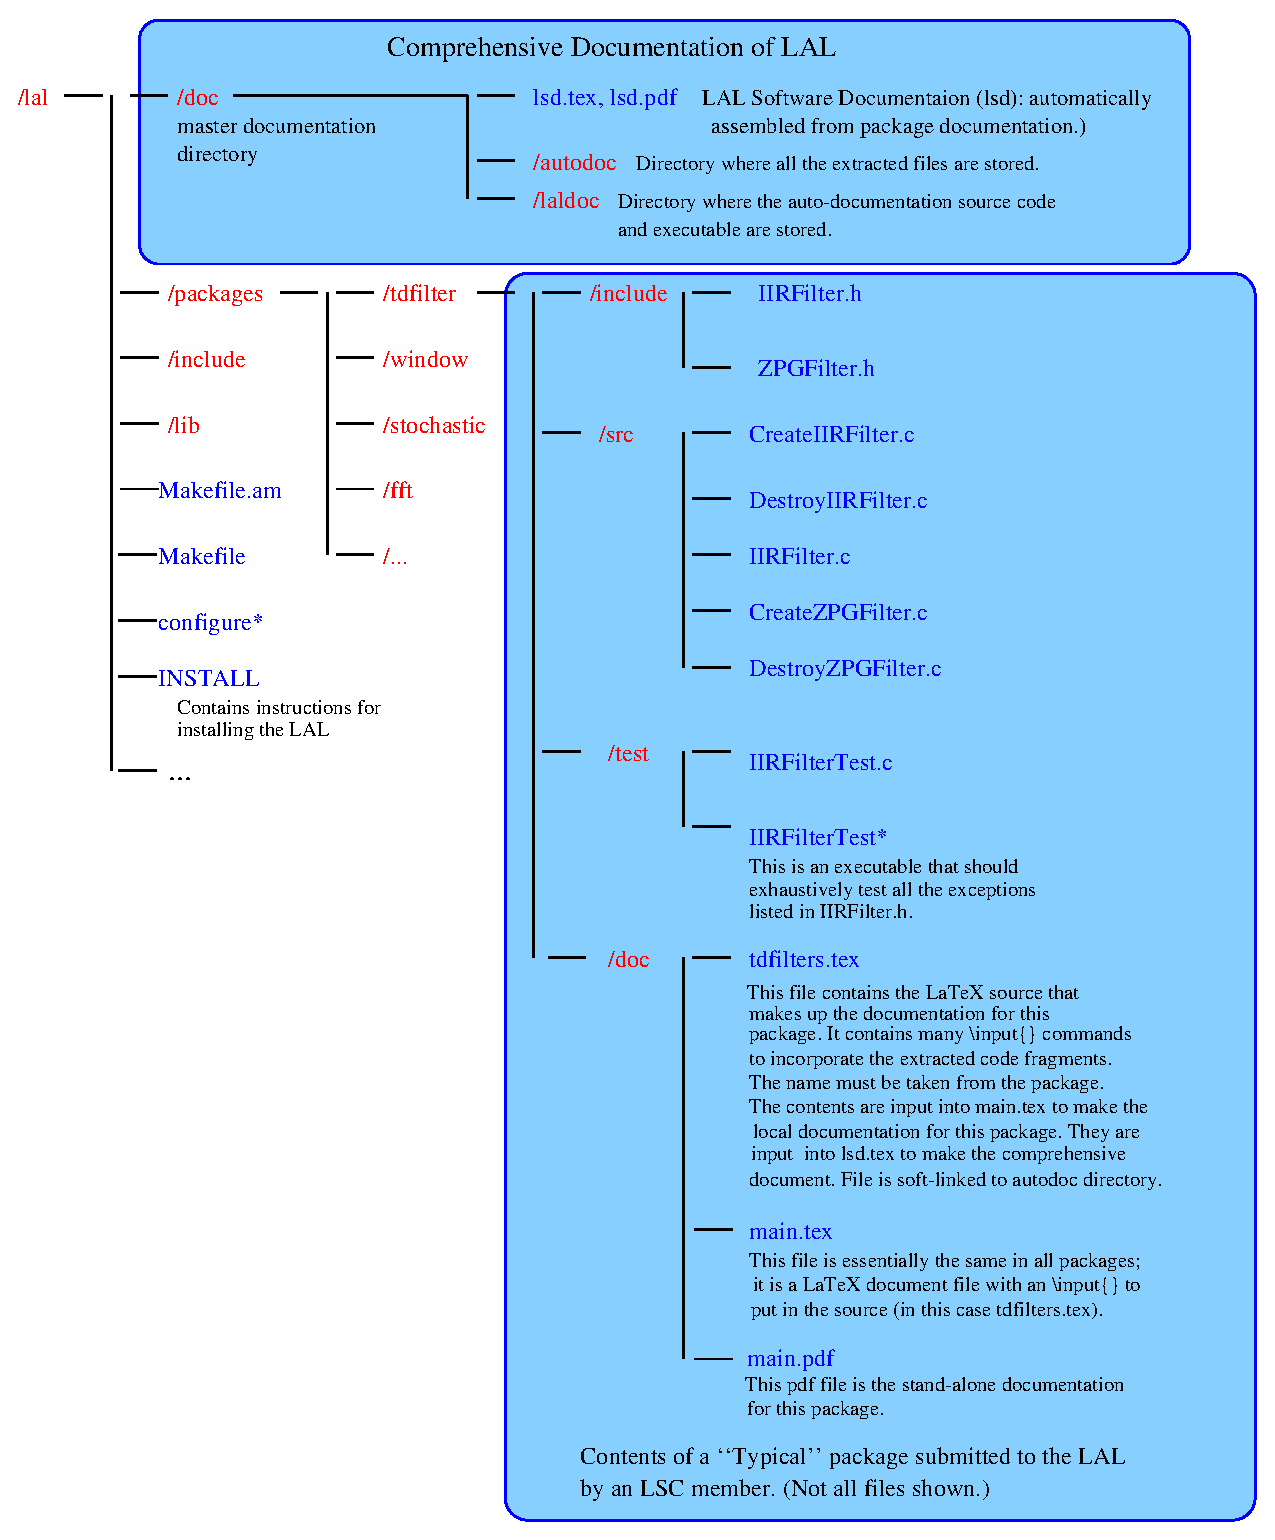
\includegraphics[width=0.9\linewidth,angle=0]{lsdFigDirStructure}

\chapter{Documenting your code}
\label{c:DocumentingCode}

Along with any code submission to the LAL library, you will need to
supply documentation. Keep in mind, the documentation, like the code,
is a {\it deliverable} and it must be written to the standard outlined
in the LAL-Spec.  This chapter gives specific instructions  on how
to meet the standard.

Also keep in mind that, unlike most code projects that physicists work
on, this code may still need to be maintained long after the author
has been denied tenure and starts working for a dot-com company.  This
puts a heavy burden on the documentation: not only should it help {\it
you} maintain {\it your} code, but it should require minimum effort
for {\it anyone} to figure out how the code works and how to fix it.
If you find yourself saying ``The easiest way for {\it me} to maintain
{\it my} code is ...'', you have missed the point.


In this chapter we discuss a few preliminaries, and give a general
outline of the documentation for a package.  Chapter
\ref{c:SamplePackage} is an example of how a the documentation for a
LAL package should be laid out. In Chapter \ref{c:laldoc} we explain
how to use the auto-documentation system ({\tt laldoc}).

\section{Use {\LaTeX}}

The documentation should be written in {\LaTeX}. This decision was made
by the LSC software committee.  The primary reason for this choice was
the need for the equation-writing capability of {\LaTeX}.

The danger in using {\LaTeX}  is that not everyone will have the same
version of {\LaTeX} installed on their machine. [Actually, this problem
might be as bad, or worse, with some other documenting tool.] Try to
help us minimize this problem by using vanilla {\LaTeX}.

Along with the LAL distribution, we supply a class file ({\tt
lal/doc/lal.sty}).  Although this is helpful and it makes thing look
nicer, it is not essential. You can remove it from the
\verb@\usepackage[]@ command in the various files and they should
still successfully {\LaTeX} without it.

\newpage
\section{The lay out of the documentation}

Most of the LDAS software is written in c++,  and therefore the
documentation is  naturally built around ``classes''.  However, the
LAL is written in c, and thus we cannot directly adopt the LDAS style
of documentation. None the less,  we try to mimic the style as close
as possible by building the LAL documentation around header files and
the modules and functions that include them.  This choice is also
natural because the hierarchical lay out of the documentation exactly
follows the hierarchy of the code.  [This is also the way books on
programming in c document the c-libraries.]

\begin{itemize}
    \vspace*{-0.1in}
    \item Documentation for the N'th package forms chapter {\large \bf N}.
    \vspace*{-0.051in}
    \begin{itemize}
        \vspace*{-0.051in}
        \item Documentation of header1.h in the package forms section
             {\large \bf N.1}.
             \begin{itemize}
                 \vspace*{-0.051in}
                 \item Documentation of Module1.1.c that
                       ``{\texttt {\#include}}'s'' header1.h
                       is in subsection {\large \bf N.1.1}.
                 \vspace*{-0.051in}
                 \item Documentation of Module1.2.c that
                       ``{\texttt {\#include}}'s'' header1.h
                       is in subsection {\large \bf N.1.2}.
                 \vspace*{-0.051in}
                 \item ... additional modules.
             \end{itemize}
        \vspace*{-0.051in}
        \item Documentation of header2.h in the package forms section.
             {\large \bf N.2}.
             \begin{itemize}
                 \vspace*{-0.051in}
                 \item Documentation of Module2.1.c that
                       ``{\texttt {\#include}}'s'' header2.h
                       is in subsection {\large \bf N.2.1}.
                 \vspace*{-0.051in}
                 \item Documentation of Module2.2.c that
                       ``{\texttt {\#include}}'s'' header2.h
                       is in subsection {\large \bf N.2.2}.
                 \vspace*{-0.051in}
                 \item ... additional modules
             \end{itemize}
        \vspace*{-0.051in}
        \item Documentation of header3.h in the package forms section.
             {\large \bf N.3}.
             \begin{itemize}
                 \vspace*{-0.051in}
                 \item ... additional modules
             \end{itemize}
        \vspace*{-0.051in}
        \item ... additional headers
    \end{itemize}
    \vspace*{-0.1in}
    \item Documentation for the N+1'th package forms chapter {\large \bf N+1}.
    \item ... additional packages
\end{itemize}

Note: Although the LAL-Spec is not rigid on the subject, it suggests
that the number of modules and functions encompassed by a header file
should be small:  only ``small sets of related functions'' should
share the same header file. This means for a given header-file
section, there shouldn't be too many module subsections.


\section{Documentation for a single package versus a comprehensive LAL manual}

The LAL-Spec mentions two distinct forms the documentation must take:
stand-alone documentation for a single package and  a comprehensive
manual (with an exhaustive index and table of contents) for the entire
LAL.  In this section we describe how we implement these two competing
documentation specifications using the same {\LaTeX} source to build
both type of documents.

The requirement of both forms of the documentation in the LAL-Spec is
not capricious: both forms of the documentation are useful. When you
are working on a single package, having a short, single-package
document is handy.  This way you won't have to wait while {\LaTeX} runs
on the complete manual for the entire LAL every time you want to see
if your equations line up. On the other hand, as the LAL code becomes
more mature and some of it starts to perform highly integrated tasks,
it will be necessary for coders to have quick access to the entire
body of documentation.

{\bf Documentation for a single package:}
The guts of the documentation for a package (e.g. {\tt sample}) should reside in the
file {\tt /lal/packages/samplepackage/doc/sample.tex}.
This file may
itself have many \verb@\input{}@ commands in it to include files that
were auto extracted from the source-code files by {\tt laldoc}.

When LAL is built, the file  {\tt sample.tex}  will be
automatically included in the file {\tt main.tex} to build the
stand alone documentation  {\tt main.pdf} for this (or any
package). In other words, the file  {\tt main.pdf} in any {\tt
lal/package/doc} is the documentation for that package.

One problem you can have when you build the documentation of a single
package is that if their are references (\verb@\ref{}@'s)  to objects
outside the package, these will be left unresolved by {\LaTeX}.  Try to
minimize these by referring to the objects by name rather than section
number.  Remember, when the comprehensive document is built, it will
have a complete index and table of contents, so the reader should be
able to easily find the documentation for the objects by name.

{\bf Comprehensive manual for the entire LAL:} In the comprehensive
documentation directory ({\tt /lal/doc}) their is a file {\tt lsd.tex}
({\tt lsd} = LAL Software Documentation). This plays essentially the
same role as {\tt main.tex} described above; however this file has an
\verb@/include{}@ statement for every package in the LAL.

\section{What about figures?}

Figures are fine. When you submit a package of code and documentation
the figures should be in the {\tt /lal/packages/mypackage/doc} directory.
Please submit two versions of the figure: an {\tt .eps} and a {\tt .pdf}.
We need both so we can build the documentation either with
{\LaTeX} or {\tt pdflatex}.

The syntax to use for putting in the figure should be something like this
\begin{verbatim}
\resizebox{0.5\textwidth}{!}{\includegraphics{myHeaderFileNameMyFig}}
\end{verbatim}
Note. Don't include the extension on the figure file name in
the \verb@\includegraphics[]{}@ command. If you leave the extension off,
whatever method you use for building the documentation automatically
looks for the appropriate file.

{\bf Naming convention for figure files:} Using the base name of the
header file as the first part of the figure file name is a good idea.
The reason: when the documentation is built, everything is {\LaTeX}ed
in  the {\tt lal/doc/autodoc} directory. There are hundreds of files there,
and  following this convention will reduce the probability of a
name-space collision.

\section{Autodocumentation and Indexing }

\subsection{Autodocumentation requirements}
There is an automatic documentation tool supplied with the LAL.  To
what extent the coders wish to use the autodocmentation system, is
largely left up to their judgment and patience. However, the
LAL-Spec require several items to be auto-extracted from the code
to include the documentation. See the LAL-Spec for the official
list, but here are some examples

\begin{itemize}
  \item[$\bullet$] {\bf Function Prototypes}
  \item[$\bullet$] {\bf Error code tables }
  \item[$\bullet$] {\bf The author and version-control information.}  This
                        should appear as footnote at the bottom of all
                        header sections, and module and test subsections.
                        This can be done with the {\LaTeX} command
                        \verb@\vfill{\footnotesize\input{MyFileHAuthVer}}@,
                        where {\tt MYFILEHAuthVer.tex} is the file where
                        the Author-Version information from {\tt MyFile.H}
                        was extracted to.  You can find examples of
                        this to mimic.
\end{itemize}

\subsection{Indexing requirements}

When this  document is built an index is also constructed. There are a few
code items that you must place in the index.
\begin{itemize}
  \item[$\bullet$] {\bf Functions} must be entered in the index, so
   users can find them. The \verb@\idx{}@ command should be right
   after the prototypes themselves are entered.  This insures the page
   number that appear in the index will be the page where the
   prototype is explained in the document.
   Use the LAL {\LaTeX} command
  \begin{verbatim}
  \idx{MyFunction()}
  \end{verbatim}
  \vspace*{-0.041in}
  \item[$\bullet$] {\bf Non LAL Data Structures}  must appear in the index.
  The LAL-Spec strongly encourages the using  LAL datatypes as the
  arguments for a function, but this isn't always possible. If you do
  use non-LAL datatypes, you must document them, and they must be
  included the index, so someone looking at your code can easily find
  the documentation.  The \verb@\idx[Type]{}@ command should be right after
  in the section where they are explained in the documentation.
  Here is an example of the LAL {\LaTeX} command you would use to get the
  name of your structure into the index.
  \begin{verbatim}
  \idx[Type]{MyType}
  \end{verbatim}
  \vspace*{-0.041in}
  \item[$\bullet$] {\bf Other Indexable Things} should also be indexed.
  If the thing is a constant variable, a constant-like macro, or an enum
  constant, index it using \verb&\idx[Constant]{thing}&.  If the thing is
  a function-like macro, index it using \verb&\idx{thing}& (which is equivalent
  to \verb&\idx[Function]{thing}&).  If it is a macro that is non-function-like
  and non-constant-like then index it using \verb&\idx[Macro]{thing}&.  If the
  thing is a variable (including function-like variables) then index it using
  \verb&\idx[Variable]{thing}&.  If the thing is a concept, then just use the
  standard \LaTeX\ command \verb&\index{thing}&.
\end{itemize}


\chapter{Package {\texttt {samplepackage}}}
\label{c:SamplePackage}

An introductory description of what is in the package.
There is no specific length limit, but $O[1]$ page seems
reasonable. Note the naming conventions for packages: all lower case.


\newpage

\section{Header {\texttt {SampleHeader1.h}}}
Put a one sentence description of the header right after the section
heading.

\subsection*{Synopsis and description}

\begin{verbatim}
#include "SampleHeader1.h"
\end{verbatim}
Since it is possible that a few modules will use the same header file
you can put a general description of what is to come here, and save
more specific comments for the module and function documentation.

\subsection*{Error conditions}
To insure that these are current with the code, a table of {\bf these
must be automatically extracted from the source code with the {\tt
laldoc} auto-documenter.} Additional explanation (if necessary) of the
error conditions can follow the table.

\subsection*{Structures}

The LAL-Spec encourages the use of LAL datatypes whenever possible,
but, if you must use  non-LAL structures, they must be documented
here.  They must also be included in the index with a
\verb@\index{sampleStruct}@ {\LaTeX} command.

\vfill{
\footnotesize{
\vspace{-1ex}
\mbox{}\marginpar{\tiny\texttt{l.1}\\\texttt{SampleHeader1.h}}
\vspace{-3ex}
\begin{verbatim}
Author: Hacker, A. Good
$Id$
\end{verbatim}
}
}

\newpage

\subsection{Module {\texttt {SampleModule1.c}}}
Put a one sentence description explaining what this module will do.
[Also, start a new page for documenting each module.]

\subsection*{Prototypes}
{\bf Function prototypes must be extracted verbatim from
the source code and ``{\verb@\input{}@}" here.}

\noindent
{\bf Every function must be placed into the index with
a \verb@\index{SampleFunction()}@ {\LaTeX} command.}

The LAL-Spec encourages modularization: ``{\it Small} sets of {\it
related} functions may grouped together into a single file.''
[Emphasis added.] Therefore, if the list of prototypes gets too long
and some aren't closely related to others, perhaps it is time to break
it up into a separate modules.

\subsection*{Description and operating instructions}
Describe the arguments of the function, and explain how to use the function.
Remember to document any non LAL {\tt structs} in the header
file documentation.

\subsection*{Algorithm}
Explanation of the algorithm.

\subsection*{Uses}
A list of all the other routines that this module uses.

\subsection*{Notes}

\subsection*{Validation Information}

This section will be formally filled in when the code is officially
validated. In the mean time, if you have timing or bench-mark testing
information, put it here.


\vfill{\footnotesize{
\vspace{-1ex}
\mbox{}\marginpar{\tiny\texttt{l.1}\\\texttt{SampleModule1.c}}
\vspace{-3ex}
\begin{verbatim}
Author: Hacker, A. Good
$Id$
\end{verbatim}
}}

\newpage

\subsection*{Program {\texttt {SampleTest.c}}}
Brief description, e.g. ``Performs tests on all routines associated with
SampleHeader.h."

\subsection*{Usage}
Show and explain the command line syntax used to run the program.

\subsection*{Description and operating instructions}
Explanation of the algorithm.

\subsection*{Exit Codes}

A table containing all the exit codes for the program.  We strongly
suggest that the exit codes be coded in exactly the same way as the
error codes in the header file.  If you do this you can use the {\tt
laldoc} Error Table tool to build a table to insert here. (See below.)
If you don't use {\tt laldoc} to make the table, please {\LaTeX} it by
hand.

The table may followed with additional explanation.

\subsection*{Uses}

A list of all the other routines that this module uses.

\subsection*{Notes}


\vfill{\footnotesize{
\vspace{-1ex}
\mbox{}\marginpar{\tiny\texttt{l.1}\\\texttt{SampleTest.c}}
\vspace{-3ex}
\begin{verbatim}
Author: Hacker, A. Good
$Id$
\end{verbatim}
}}


\chapter*{References}

This should be a stand-alone bibliography for the references used in
this package only.  We recognize there may be entries that are
repeated in other packages and there are more clever ways to do this,
but this seems to be the simplest.

\chapter*{Index}
The index for the Package {\tt samplepackage} should start on a new
page.  The \verb@\printindex@ command should be in the {\tt main.tex}
file, because we only want this index to appear in the stand-alone
documentation for this package.  When we the comprehensive
documentation is built, only the all-encompassing index will appear
at the end of the entire document.

\part{LALDoc: Automated Documentation}

\chapter{The automatic documentation system}
\label{c:laldoc}

We will first describe the code parser that sifts through the source
code and extracts the parts that are to be incorporated into the
documentation. Then we describe how the documentation is automatically
built when the LAL is installed.

\section{A four step introduction to the code parser {\texttt {laldoc}}}

\noindent
These four-step instructions are also outlined in the file
{\tt /lal/doc/laldoc/README}.

\begin{itemize}
\item[(1)] Copy the executable ({\tt /lal/doc/laldoc/laldoc})
and the  sample input file ({\tt /lal/doc/laldoc/LalDocDemo.h}) to an
empty  {\tt /home/alice/junk} directory.
\item[(2)] In {\tt /home/alice/junk}
run the command ``\verb@./laldoc LalDocDemo.h Errors.out@''
\item[(3)] {\LaTeX} the file {\texttt {LalDocDemo\_LaTeX\_This\_File.tex}}.
\item[(4)] Read the  document created in step 3
({\texttt {LalDocDemo\_LaTeX\_This\_File.dvi}}) . It will explain how
the various debris files were created from the original source file
and how they were input to make the document.  If you follow your
nose,  you will see exactly what  {\texttt {laldoc}} does and how it
works.  Also, make sure you look at the file {\tt Errors.out}.
\end{itemize}

\section{Brief Description of the parser {\texttt {laldoc}} }

The purpose of the auto-documentation procedure we are using with the
LAL is to adhere the common wisdom: ``keep the documentation close to
the code''.  The system is built around a a code
parser {\tt laldoc} that allows LAL programmers automatically extract fragments of
code or comments from the source files and include them in their
documentation.  This is done in such a way that if the fragment in the
source code is modified, then the change is automatically incorporated
into the documentation the next time the document is built.

This extraction is  accomplished by having the programmer surround the
fragments of code or comments he or she wishes to incorporate in the
document with key-words.  Currently, we only have three pairs of
key-words, so the learning curve is flat and short! The source code
(the .c and .h files) is then parsed and the fragments written to
storage files.  (The key-word also includes a space for user-specified file name
where the fragment will be stored.)  When you write your documentation simply
use the {\LaTeX} command \verb@\input{}@ to put the contents of the
storage file in the document where you need it.

When you install the LAL on your machine, the parser is automatically
run on all {\tt .c} and {\tt .h} files. The extracted files are
stuffed into the directory {\tt lal/doc/autodoc/}.  If you have
installed the LAL software package, take a look at the contents of
{\tt lal/doc/autodoc/}. Their are dozens of extracted files their.

\subsection{ The {\texttt {laldoc}} command line }
The full functionality of the command line is:
\begin{verbatim}
     laldoc inputFile.c errorFile /home/alice/errorDir/ /home/alice/inputDir/
\end{verbatim}
\noindent
The zeroth command line argument is the executable itself.
The first argument is the input file name, the second is an error reporting
file, the third argument is the directory where the error file will be
written, and the fourth is the directory where {\tt laldoc} will look
for the input file.  The third and the fourth arguments are optional.


\subsection{ The three {\texttt {laldoc}} environments }

One general comment about the  {\texttt {laldoc}} environments:
None of the text on the line with the opening key-word or on the
line with the closing key-word will be extracted.

\begin{description}
\item[$\bullet$ ]
The verbatim environment is opened key-word
{\verb@<lalVerbatim file="myVerbatimJunk">@}  and closed with the key-word
{\verb@</lalVerbatim>@}. The material between the two key-words will
be wrapped in a {\LaTeX} {\tt verbatim} environment for later
inclusion.  This is useful for including such things as a function
prototypes or data structures: they will appear ``verbatim'' in the
documentation.  When the information is included with {\tt
<lalVerbatim>} {\tt laldoc} supplies a small {\tt marginpar} gives the
source-file name and line number where the snippet came from.
\vspace*{-0.05in}
\item[$\bullet$ ]
The {\LaTeX} environment is opened and closed with the key-words
{\verb@<lalLaTeX file="myLatexJunk">@}  and {\verb@</lalLaTeX>@}. This is
used to write {\LaTeX} in the source-code. The material between the two
key-words is stored in a file {\tt myLatexJunk.tex}.  This allows (not
recommended) a programmer to put large sections of {\LaTeX} prose in the
source code.
\vspace*{-0.05in}
\item[$\bullet$ ]
The error-table environment.  There is a special environment for
translating the source code that assign the error codes and messages
directly into a {\LaTeX} table. All you need to do is wrap the code
between the key-words {\verb@<lalErrTable file="myErrTabJunk">@} and
{\verb@</lalErrTable>@}.  This insures that if an error code is added
in the source, it will automatically be added to the documentation.
\vspace*{-0.051in}
\end{description}

\subsection{ How {\texttt {laldoc}} handles the output files}

{\bf Default file names:} In any of the {\texttt {laldoc}} environments,
if you do not specify an output file in the opening key-word line,
{\texttt {laldoc}} will assign one automatically. The file name will
be constructed from the input file name, e.g. if the input
is  {\tt MyHeader.h}, the default output will be {\tt MyHeaderH.tex}.

{\bf Appending to files:}
If the output file doesn't already exist, {\texttt {laldoc}} will
create it.  If the output file already exists, {\texttt {laldoc}} will
append to it.  When the environment-closing key-word is encountered,
the output file is closed.

Although this is a fairly obvious feature, it is quite useful.  For
example, the function prototypes in a module don't appear together in
the source, but they should appear together in the documentation.
With {\texttt {laldoc}} this is easy to accomplish. In your source
code when you encounter each prototype that must be captured for
inclusion, use the same file name for the extraction, i.e surround
each prototype with
the pair {\verb@<lalVerbatim file="MyModuleCPrototypes">@}  and
{\verb@</lalVerbatim>@}.  Each prototype will be appended to the file
{\tt MyModuleCPrototypes.tex}, and separate margin pars will tell
exactly where each came from.





\section{Examples of how to use the three environments in {\texttt {laldoc}} }

As with most things computer, the best way to learn how use the auto
documenter is to snoop around the source tree and find some examples,
and then try a few things.  The source code and the executable for the
parser ({\tt laldoc}), are in the directory {\tt lal/doc/laldoc}.  The
directory also has a README file that give some nuts-n-bolts
instructions on how to use the parser.  This sections gives the basics
of what you can do.


\subsection{The {\texttt {<lalVerbatim>} }  environment }

As an example, look at the code fragment in the source file
\texttt{lal/packages/tdfilter/src/CreateZPGFilter.c}.

\begin{verbatim}
    /* <lalVerbatim file="CreateZPGFilterCP"> */
    void CreateCOMPLEX8ZPGFilter(LALStatus          *stat,
                                 COMPLEX8ZPGFilter **output,
                                 INT4              numZeros,
                                 INT4              numPoles)
    /* </lalVerbatim> */
\end{verbatim}
When {\tt laldoc} parses the source file, it produces the following
output in the file {\tt CreateZPGFilterCP.tex}

\begin{verbatim}

\vspace{-1ex}
\mbox{}\marginpar{\tiny\texttt{l.51}\\\texttt{CreateZPGFilter.c}}
\vspace{-3ex}
(backslash)begin{verbatim}
void CreateCOMPLEX8ZPGFilter(LALStatus         *stat,
                             COMPLEX8ZPGFilter **output,
                             INT4              numZeros,
                             INT4              numPoles)
(backslash)end{verbatim}
\end{verbatim}

This is then included in the {\LaTeX} documentation with an
\verb@\input{CreateZPGFilterCP}@ command, yielding the following
output:

\vspace{-1ex}
\mbox{}\marginpar{\tiny\texttt{l.51}\\\texttt{CreateZPGFilter.c}}
\vspace{-3ex}
\begin{verbatim}
void CreateCOMPLEX8ZPGFilter(LALStatus         *stat,
                             COMPLEX8ZPGFilter **output,
                             INT4              numZeros,
                             INT4              numPoles)
\end{verbatim}

The {\tt marginpar} on the far right tells the line number and file
name where the fragment came from.

{\bf Note the naming convention used for the file where the extracted
code was stored: the base name comes from the file where it was
extracted (here {\texttt {CreateZPGFilter}}), followed by a ``C'' (in
this case to denote that it came from the .c file).  {\Large {Use This
Naming Convention!}} This will avoid most name-space collisions.}  In
this case,  the the ``P'' is for function {\it prototype}.


\subsection{The {\texttt {<lalLaTeX>} } environment }

The {\texttt {<lalLaTeX>} } environment works much the same
was as the {\texttt {<lalVerbatim>} } environment. The distinction
being that the extracted material should be valid {\LaTeX} ready
for insertion into a {\LaTeX} file.

In the {\texttt {<lalLaTeX>}} environment, leading ``*'''s on a line
will be stripped out by {\tt laldoc}. This is to accommodate the common
practice in c of putting leading ``*'''s on comment lines.  The way
this is done is {\tt laldoc} checks to see if the first non blank
character on the line is a ``*''. If it is, then it is replaced by
blank when the line is written to the output file. The leading
blanks are ignored when the file is {\LaTeX}ed.


\subsection{The {\texttt {<lalErrTable>} } environment, for printing
a table of the error codes and warnings.}

See the example in Chapter \ref{c:CodingNotes}.


\section{How the documentation is automatically built}

Some of the documentation (perhaps most of it)  for a package is in
the source files awaiting extraction.  The rest of the documentation
for the package is in the {\tt lal/packages/mypackage/doc/} directory.
How does it all get pulled together to make a coherent document?  The
short version of the explanation is that all the necessary files
either exist in, or are copied to, or are linked to the directory {\tt
lal/doc/autodoc/}, then {\LaTeX} is run in the {\tt autodoc/} directory
and important results are moved back.  You can see the specifics of
how this happens (and how to modify it for your own use) if you examine
the contents of the {\tt Makefile.am}'s in the various {\tt doc/}
directories.

When  you type {\tt make dvi} during the installation, a chain of
events takes place. First, the {\tt laldoc} parser is run in each
source directory ({\tt src}, {\tt include} and {\tt test}) in all the
packages.  The documentation snippets are culled out of the source
files and stuffed into files in {\tt /lal/doc/autodoc} directory. When
this is complete, the stand-alone documentation is built one directory
at time.  First, links from the {\tt .tex}, {\tt .eps} and {\tt .pdf}
files to the {\tt autodoc} directory are established.  Then the {\tt
main.tex} file is copied from the package's  {\tt /doc} directory to
the {\tt autodoc} directory. Then {\tt main.tex} is {\LaTeX}ed
(actually, we run {\tt pdflatex}). When this is complete, {\tt
main.pdf}  and {\tt main.tex} are moved back the package's {\tt doc}
directories.  This is repeated for each package.

After the documentation for the individual packages is built, then the
comprehensive documentation is built in essentially the same way.  The
file {\tt /lal/doc/lsd.tex} is copied to the {\tt autodoc} directory
and {\LaTeX}  ({\tt pdflatex}) is run on it. Then  {\tt lsd.tex} and
{\tt lsd.pdf} are moved back to the {\tt doc} directory.



\backmatter
\pagebreak
\renewcommand{\bookname}{\relax}
\addcontentsline{toc}{book}{Index}%
\nopagebreak
\printindex

\end{document}
